\documentclass[MScCS]{uccthesis}

% Extra packages needed for algorithms, tables, and floats
\usepackage{algorithm}
\usepackage{algpseudocode}
\usepackage{tabularx}
\usepackage{threeparttable}
\usepackage{multirow}
\usepackage{amssymb}
\usepackage{float}
\usepackage{placeins}
\usepackage{caption}
\usepackage{array}
\usepackage{subcaption}
\usepackage{textcomp}
\usepackage{csquotes}
\usepackage{silence}
\WarningFilter{minitoc(hints)}{W0024}
\WarningFilter{minitoc(hints)}{W0030}
\WarningFilter{minitoc(hints)}{W0023}
\WarningFilter{minitoc(hints)}{W0028}

\ExecuteBibliographyOptions{doi=true,url=true,isbn=false}
\usepackage[hidelinks]{hyperref}
\hypersetup{
  colorlinks=true,
  linkcolor=blue,
  citecolor=blue,
  urlcolor=blue
}

\renewcommand{\chapterautorefname}{Chapter}
\renewcommand{\sectionautorefname}{Section}
\renewcommand{\subsectionautorefname}{Section}
\renewcommand{\figureautorefname}{Figure}
\renewcommand{\tableautorefname}{Table}
\renewcommand{\algorithmautorefname}{Algorithm}

\dominitoc
\dominilof
\dominilot
\hbadness=10000
\hfuzz=1000pt

\addbibresource{references.bib}

\title{EnsembleNet: Statistically Validated Demand Forecasting and Constraint-Aware Ride Pooling for Urban Shared Taxi Systems}
\author{Vishal Sharma}
\supervisor{Dr Md Noor-A-Rahim}
\secondreader{TBD}
\date{August 2026}

\abstract{Urban taxi systems face mounting pressure to reduce congestion, cost, and emissions, yet existing studies address demand forecasting and ride pooling in isolation and rarely apply rigorous statistical validation. This thesis introduces a unified data-driven framework combining ensemble-based demand forecasting with a multi-criteria ride pooling algorithm, evaluated on New York City Yellow Taxi records. A novel LR-LSTM hybrid architecture decomposes demand into a linear trend and a non-linear residual, and six ensemble strategies are benchmarked against eight individual estimators under a strictly chronological train-test protocol, with a Friedman test confirming statistical significance of observed differences. The ride pooling component enforces temporal, spatial, directional, and detour constraints, with city-scale economic and environmental impact quantified via bootstrap estimation. Results show that the Stacking ensemble substantially outperforms the established LR-LSTM benchmark, and the pooling algorithm delivers meaningful reductions in per-trip cost and carbon emissions, demonstrating a statistically validated and deployable approach to shared taxi system management.}

\acknowledgement{I thank Dr Md Noor-A-Rahim for his supervision and guidance throughout this project. I also thank MD All Moon Tasir for co-supervision and support.}

\renewcommand\addToFrontMatter[0]{%
}

\begin{document}

% ============================================================
\chapter{Introduction}
\label{ch:introduction}
% ============================================================

\section{Background}

Urbanisation is reshaping mobility at an unprecedented pace: the United Nations projects that 68\% of the world's population will reside in cities by 2050~\parencite{un2018wup}, intensifying congestion, greenhouse gas emissions, and demand for scalable, on-demand transport.  In New York City alone, taxis and ride-hailing vehicles account for hundreds of millions of trips annually, contributing substantially to urban congestion and vehicular emissions~\parencite{taxinyc_dataset}.  Shared-ride taxi services sit at the intersection of these pressures, capable of door-to-door coverage that mass transit cannot provide, yet environmentally costly when vehicles carry a single passenger.  Realising the potential of shared taxis therefore requires two complementary capabilities: accurate \emph{demand forecasting}, enabling operators to pre-position vehicles and reduce idle mileage, and effective \emph{ride pooling}, so that compatible trips share a vehicle and reduce per-passenger cost and emissions.

Taxi demand forecasting is a spatio-temporal prediction problem of significant practical complexity.  Demand varies sharply by time of day, day of week, weather conditions, and geographic zone, requiring models that can capture both linear trends and non-linear interaction effects simultaneously.  Ensemble methods have shown consistent superiority in tabular prediction tasks~\parencite{breiman2001rf,chen2016xgboost,wolpert1992stacking}, yet no prior study has systematically compared a comprehensive suite of ensemble strategies on the same spatio-temporal demand task with non-parametric statistical validation.  Ride pooling, independently, requires matching algorithms that balance pool rate, per-trip savings, and realistic passenger-acceptance constraints, yet most operational studies either report theoretical upper bounds~\parencite{santi2014quantifying} or fleet-level outcomes without pairwise economic quantification~\parencite{alonso2017demand}.

\section{Research Gap}

Existing literature has explored each capability in isolation.  Demand-forecasting studies, from early data-driven baselines~\parencite{dia2002object} and streaming prediction approaches~\parencite{moreira2013predicting} to deep spatio-temporal networks~\parencite{zhang2017deep,xu2017realtime,kim2020hybrid}, demonstrate steady accuracy gains, yet rarely validate whether observed improvements across model classes are statistically significant.  Ride-pooling analyses such as the shareability network of~\parencite{santi2014quantifying} and the real-time framework of~\parencite{alonso2017demand} report theoretical upper bounds rather than evaluating operational algorithms under realistic passenger-acceptance constraints.  Neither body of work simultaneously quantifies economic and environmental impact at both the trip and city scale.  This thesis addresses all three gaps within a single, reproducible framework evaluated on two years of publicly available New York City Yellow Taxi records.

\section{Objectives and Contributions}

This thesis addresses these gaps through three contributions.

First, a systematic ensemble benchmarking study evaluates fourteen forecasting models on NYC Yellow Taxi data under strictly chronological splits.  A Friedman non-parametric test confirms that observed differences across model classes are statistically significant, with Stacking achieving R\textsuperscript{2}~=~0.9922 and MAPE~=~10.19\%, establishing a strong upper bound for spatio-temporal taxi demand prediction.

Second, a novel LR-LSTM hybrid architecture is proposed in which a Linear Regression stage extracts the deterministic demand trend and an LSTM stage models the non-linear residuals.  An XGBoost-LSTM variant is introduced alongside for comparison, allowing the contribution of each residual-modelling strategy to be isolated and quantified.

Third, a constraint-aware ride pooling algorithm is developed that applies five cascading compatibility filters reflecting realistic passenger-acceptance requirements.  The algorithm achieves a 16.06\% pool rate on 106,055 sampled trips, with projected annual savings of USD~28.7~million and approximately 3{,}370~tonnes of CO\textsubscript{2} for New York City scaled from the sample using the verified 2015 NYC Yellow Taxi annual volume of $\approx$146M trips~\parencite{nyc_opendata_2015}, factor $\approx 1{,}377$, validated through bootstrap resampling with 10,000 iterations.

\section{Thesis Structure}

The remainder of this thesis is organised as follows.  \autoref{ch:related} reviews related work.  \autoref{ch:methods} describes the dataset, preprocessing, spatial clustering, feature engineering, and the ride pooling algorithm.  \autoref{ch:framework} presents the proposed EnsembleNet framework, including individual model architectures, the LR-LSTM hybrid, and the six ensemble strategies.  \autoref{ch:metrics} defines the evaluation metrics.  \autoref{ch:results} reports experimental results and discusses implications, limitations, and future work.  \autoref{ch:conclusion} concludes.

\autoref{fig:intro} presents a high-level overview of the two complementary subsystems that constitute the proposed framework.  The left panel captures the spatial dimension: raw pickup coordinates are partitioned into $K{=}40$ data-driven clusters using MiniBatch KMeans, converting a continuous geographic space into a tractable set of neighbourhood-level demand zones.  Within each zone, demand is aggregated into 10-minute temporal bins, producing a feature matrix that is then enriched with lag features, time-of-day cyclical encodings, weather measurements, and public holiday indicators.  The right panel captures the operational dimension: for any 5-minute window of incoming trips, pairs of rides are evaluated against five cascading filters covering time proximity, origin proximity, destination proximity, route direction alignment, and maximum detour ratio.  Only pairs clearing all five filters receive a weighted compatibility score; a greedy matching pass then assembles the highest-scoring pairs into shared rides.  The two subsystems are designed to operate sequentially in production: demand forecasts inform vehicle pre-positioning, while the pooling algorithm processes the resulting trip requests in real time.  Together they address both the supply-side optimisation problem and the demand-side coordination problem that characterise shared urban mobility.

\begin{figure}[t]
  \centering
  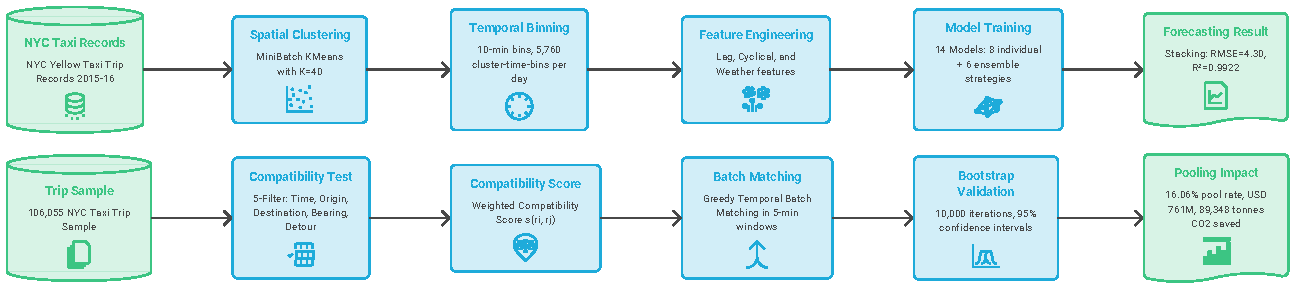
\includegraphics[width=\textwidth, height=0.45\textheight, keepaspectratio]{Figures/Intro.pdf}
  \caption{Overview of the proposed EnsembleNet framework for NYC shared taxi systems. The left panel shows data-driven spatial clustering of pickup locations into $K{=}40$ demand zones and the temporal demand patterns observed within each zone. The right panel depicts the multi-criteria ride pooling matching pipeline, showing how compatible trip pairs are identified and how cost and environmental savings are estimated.}
  \label{fig:intro}
\end{figure}

% ============================================================
\chapter{Related Work}
\label{ch:related}
% ============================================================

Prior research on urban taxi systems can be organised across three threads: demand forecasting, ride pooling, and ensemble methods.

Early demand forecasting methods relied on ARIMA variants, which capture linear temporal patterns but cannot encode spatial correlations.  Moreira-Matias et al.~\parencite{moreira2013predicting} demonstrated streaming-based demand prediction from real-time GPS data, while Lv et al.~\parencite{lv2015traffic} showed that deep learning outperforms time-series baselines on large-scale traffic flow data.  Zhang et al.~\parencite{zhang2017deep} introduced ST-ResNet, which treats citywide demand grids as image sequences processed by deep residual convolutions.  Xu et al.~\parencite{xu2017realtime} confirmed that LSTM networks outperform feed-forward architectures for real-time NYC taxi demand by exploiting sequential autocorrelation.  Ma et al.~\parencite{ma2015long} and Ke et al.~\parencite{ke2017short} further validated LSTM superiority for transportation speed and ride-hailing demand tasks respectively.  Kim et al.~\parencite{kim2020hybrid} proposed the LR-LSTM model, a two-stage hybrid achieving R\textsuperscript{2}~=~0.572 and MAPE~=~15.2\% on Murray Hill, NYC, which serves as the primary benchmark in this study.  Liu et al.~\parencite{liu2021epidemic} reported XGBoost attaining R\textsuperscript{2}~=~0.984 on NYC Yellow Taxi data, highlighting distributional shift as a key challenge.  Guo et al.~\parencite{guo2019attention} proposed attention-based spatio-temporal graph convolutional networks, demonstrating that graph structures capture inter-zone dependencies more effectively than grid-based methods.  Li et al.~\parencite{li2018diffusion} introduced DCRNN, which encodes directional diffusion on road graphs, though this requires detailed road-topology data unavailable in the present study.  Zhou et al.~\parencite{zhou2018predicting} applied attention mechanisms to multi-step citywide passenger demand prediction.  More recently, Liu et al.~\parencite{liu2023staeformer} proposed STAEformer, which augments a vanilla Transformer with spatio-temporal adaptive embeddings and achieves state-of-the-art results on standard traffic speed and flow benchmarks including METR-LA and PEMS-BAY; because STAEformer targets road-network speed prediction rather than zone-level pickup-count forecasting, direct numerical comparison with the present study is not feasible, but it represents the current frontier of spatio-temporal deep learning and motivates future work on graph-based demand forecasting.

On the ride pooling side, Santi et al.~\parencite{santi2014quantifying} established via shareability network analysis that ride consolidation can achieve up to $\sim$40\% cumulative trip-length reduction across the NYC fleet under idealised conditions, providing a theoretical upper bound for any operational algorithm.  Alonso-Mora et al.~\parencite{alonso2017demand} developed a real-time framework serving nearly the entire NYC demand with 15\% fewer vehicles via dynamic trip-vehicle assignment.  Agatz et al.~\parencite{agatz2012ridesharing} reviewed dynamic ridesharing optimisation and concluded that greedy heuristics offer a practical balance between solution quality and tractability.  Furuhata et al.~\parencite{furuhata2013ridesharing} identified four matching criteria, namely temporal flexibility, spatial proximity, directional compatibility, and willingness to share, which directly inform the five-filter design of Algorithm~\ref{alg:ride_pool}.  Tang et al.~\parencite{tang2018joint} characterised the joint distribution of taxi passenger counts and waiting times, providing empirical support for the 8-minute temporal threshold used in this study.

In the ensemble learning literature, Wolpert~\parencite{wolpert1992stacking} formalised stacked generalisation, showing that a meta-learner trained on out-of-fold predictions reduces overfitting.  Breiman~\parencite{breiman2001rf} introduced Random Forests and Friedman~\parencite{friedman2001gbm} developed Gradient Boosting Machines, establishing the foundations for the ensemble strategies evaluated here.  Chen and Guestrin~\parencite{chen2016xgboost} refined boosting with regularisation and sparse-matrix support to produce XGBoost.  Zheng et al.~\parencite{zheng2020hybrid} demonstrated hybrid deep learning and gradient boosting for traffic speed prediction, motivating the XGBoost-LSTM hybrid in this study.  No prior work has systematically compared six ensemble strategies on the same spatio-temporal demand task with non-parametric statistical validation.  \autoref{tab:litreview} summarises representative prior work and the gaps that this study addresses.

\begin{table}[t]
\centering
\caption{Summary of representative prior work on taxi demand forecasting, ride pooling, and ensemble methods. Stat.\ Val.\ denotes non-parametric cross-model significance testing. Pooling denotes an operational ride-pooling component evaluated in the same study.\label{tab:litreview}}
\small
\begin{tabular}{@{}p{2.0cm}p{1.35cm}p{1.9cm}p{2.2cm}p{2.3cm}cc@{}}
\toprule
\textbf{Study} & \textbf{Domain} & \textbf{Dataset} & \textbf{Method} & \textbf{Key Result} & \textbf{Stat.\ Val.} & \textbf{Pooling} \\
\midrule
Kim et al.~\parencite{kim2020hybrid} & Demand & NYC Yellow Taxi & LR-LSTM hybrid & R\textsuperscript{2}=0.572; MAPE=15.2\% & No & No \\
Xu et al.~\parencite{xu2017realtime} & Demand & NYC Taxi & LSTM RNN & MAPE~$\approx$12.5\%; real-time & No & No \\
Zhang et al.~\parencite{zhang2017deep} & Crowd flow & Beijing / NYC & ST-ResNet & Deep residual grids & No & No \\
Liu et al.~\parencite{liu2021epidemic} & Demand & NYC Yellow Taxi & XGBoost & R\textsuperscript{2}=0.984; COVID shift & No & No \\
Yao et al.~\parencite{yao2018deeptraffic} & Demand & NYC Taxi & DeepMVST & Multi-view ST forecast & No & No \\
Zhang et al.~\parencite{zhang2023deeptrip} & Trip pred. & GPS traces & DeepTrip & 81\% next-origin accuracy & No & No \\
Li et al.~\parencite{li2018diffusion} & Traffic & Road network & DCRNN & Directed diffusion GNN & No & No \\
Santi et al.~\parencite{santi2014quantifying} & Pooling & NYC Taxi & Shareability networks & $\sim$40\% length reduction bound & No & Yes \\
Alonso-Mora et al.~\parencite{alonso2017demand} & Pooling & NYC Taxi & Dynamic assignment & 98\% demand; 15\% fewer vehicles & No & Yes \\
Agatz et al.~\parencite{agatz2012ridesharing} & Pooling & Various & Optimisation survey & Greedy tractability trade-off & No & Yes \\
Furuhata et al.~\parencite{furuhata2013ridesharing} & Pooling & Various & Matching criteria survey & Four operational criteria & No & Yes \\
Wolpert~\parencite{wolpert1992stacking} & Ensemble & Synthetic & Stacked generalisation & OOF meta-learning & No & No \\
\textbf{This work} & Both & NYC Yellow Taxi & 14-model ensemble + 5-filter pooling & Stacking R\textsuperscript{2}=0.9922; 16.06\% pool rate & Yes & Yes \\
\bottomrule
\end{tabular}
\end{table}

% ============================================================
\chapter{Methods and Materials}
\label{ch:methods}
% ============================================================

This chapter describes the full experimental methodology, covering the dataset and its preprocessing, spatial clustering, feature engineering, and the ride pooling algorithm.  \autoref{fig:pipeline} illustrates the complete processing pipeline.

\begin{figure}[t]
  \centering
  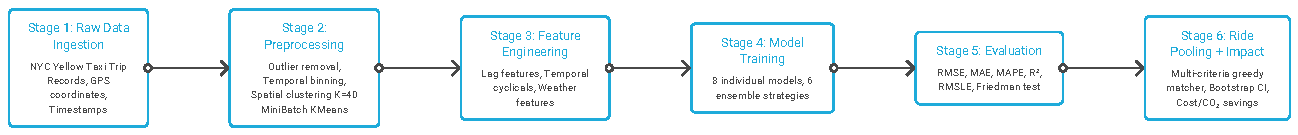
\includegraphics[width=\textwidth, height=0.52\textheight, keepaspectratio]{Figures/complete_pipeline.pdf}
  \caption{Complete research pipeline from raw data to city-scale impact: data ingestion, outlier removal, spatial clustering, temporal binning, feature engineering, model training and evaluation, ride pooling matching, bootstrap validation, and economic and CO\textsubscript{2} impact projection.}
  \label{fig:pipeline}
\end{figure}

\autoref{fig:pipeline} traces the end-to-end data flow through six sequential stages.  Stage~1 ingests the raw NYC Yellow Taxi Trip Records and applies coordinate boundary filtering, duration filtering, and fare filtering to remove implausible records.  Stage~2 constructs spatial zones via MiniBatch KMeans on a stratified 5\% sample of pickup coordinates, choosing $K{=}40$ as the cluster count validated by inertia elbow, silhouette score, and downstream prediction RMSE criteria.  Stage~3 aggregates trips into 10-minute bins per cluster and engineers the full feature set described in \autoref{tab:features}.  Stage~4 trains all 14 models under a strictly chronological 80/20 split and evaluates them across five metrics.  Stage~5 applies the multi-criteria ride pooling algorithm to a 106,055-trip sample, computing compatibility scores and greedy matches within 5-minute windows.  Stage~6 applies bootstrap resampling over 10,000 iterations to produce 95\% confidence intervals for pool rate, savings, and compatibility metrics, and scales the sample estimates to full NYC annual volume for city-wide impact projection.  Each stage is implemented as a modular Python notebook, facilitating independent validation and extension.


\section{Dataset}

This study uses the publicly available NYC Yellow Taxi Trip Records~\parencite{taxinyc_dataset} hosted on Kaggle.  The training split covers January 2015, comprising approximately 12.7 million trips, and the test split covers January to March 2016, comprising approximately 34 million trips.  Each record includes pickup and drop-off timestamps, GPS coordinates, passenger count, trip distance, and fare information.  \autoref{tab:dataset} summarises the dataset.

\begin{table}[t]
\centering
\caption{NYC Yellow Taxi dataset statistics.\label{tab:dataset}}
\begin{tabularx}{\textwidth}{>{\raggedright\arraybackslash}X r}
\toprule
\textbf{Attribute} & \textbf{Value} \\
\midrule
Training period & January 2015 \\
Testing period  & January--March 2016 \\
Approximate training trips & 12.7 million \\
Approximate test trips & 34 million \\
Spatial bounding box (lat) & 40.58 -- 40.92 \\
Spatial bounding box (lon) & $-$74.15 -- $-$73.70 \\
Features per record & 19 \\
\bottomrule
\end{tabularx}
\end{table}

\subsection{Chronological Train-Test Split}
A key methodological requirement for time-series data is that the training set precedes the test set in calendar time.  The split is \emph{strictly chronological}: the training set is drawn entirely from January 2015 and the test set from January--March 2016, separated by an 11-month gap.  At the aggregated feature-matrix level, records are sorted ascending by \texttt{datetime\_bin} and split at 80\% using \texttt{train\_test\_split(shuffle=False)}, ensuring no lag-feature from the future leaks into training.

The 11-month gap between training and test periods is a deliberate design choice rather than an artefact of data availability.  A contiguous split -- for example, training on January through October 2015 and testing on November through December 2015 -- would evaluate models on demand patterns from the same seasonal period as the training data, creating an optimistic estimate of generalisation.  By spanning the gap to January--March 2016, the evaluation requires the models to generalise across a full seasonal cycle: patterns learned in a winter month must transfer to demand conditions in a subsequent winter that may differ in weather severity, fare structure, or local event schedule.  This design tests out-of-distribution generalisation in the sense most relevant to operational deployment, where a model trained on historical data must perform reliably months into the future without retraining.  The 11-month gap also ensures that any year-on-year shifts in NYC taxi demand, including the growing competition from ride-hailing platforms observed from 2015 to 2016, are reflected in the evaluation, providing a conservative and realistic bound on expected model performance.

\section{Data Preprocessing}

Two preprocessing steps are applied to the raw trip records before feature engineering: coordinate, duration, and fare filtering to remove implausible observations, and external feature augmentation to enrich each record with weather and calendar context.

\subsection{Outlier Removal}
Trips with GPS coordinates outside the NYC bounding box, defined as latitude 40.5774 to 40.9176 and longitude $-$74.15 to $-$73.7004, are discarded.  Trips shorter than one minute or longer than 12 hours are removed as implausible.  Fare amounts below the NYC minimum of \$2.50 are also filtered.  Memory is optimised by downcasting numeric columns to their minimum compatible dtype, reducing RAM usage by approximately 45\%.

\subsection{External Features}
The trip records are augmented with two additional external data sources.  Daily weather data, comprising temperature in degrees Fahrenheit, precipitation in inches, snowfall in inches, and a categorical condition label, are sourced from NOAA for the corresponding dates.  A binary public holiday indicator for US federal holidays is derived from the \texttt{holidays} Python library and merged by date.

\section{Spatial Clustering and K Selection}
\label{sec:spatial}

Rather than imposing an administrative zone system, data-driven spatial zones are constructed using MiniBatchKMeans clustering~\parencite{kmeans_mini} applied to 5\% of pickup coordinates.  Given pickup coordinates $\{\mathbf{p}_i\}_{i=1}^{n}$, the algorithm minimises the within-cluster sum of squares in \eqref{eq:kmeans}, assigning each trip to the nearest of $K$ centroids $\{\boldsymbol{\mu}_k\}_{k=1}^{K}$:
\begin{equation}
  \min_{\{\boldsymbol{\mu}_k\},\,\{S_k\}}
  \sum_{k=1}^{K}\sum_{\mathbf{p}_i\in S_k}
  \bigl\|\mathbf{p}_i - \boldsymbol{\mu}_k\bigr\|_2^{2}.
  \label{eq:kmeans}
\end{equation}
A total of $K=40$ clusters are adopted, yielding neighbourhood-level spatial granularity.

The decision to derive spatial zones from data rather than adopt an administrative boundary system such as NYC community districts or taxi zone polygons reflects a methodological preference for demand-aligned granularity.  Administrative zones vary widely in geographic extent and trip density: Manhattan community districts encompass both high-volume commercial cores and low-volume residential blocks within a single polygon, averaging out the sharp spatial heterogeneity that drives dispatch decisions.  Data-driven clustering, by contrast, partitions the coordinate space so that each centroid represents a locally homogeneous demand region, allowing the model to learn neighbourhood-specific pickup patterns without being constrained by political boundaries that may bear little relation to actual trip origins.  MiniBatch KMeans is chosen over standard KMeans for computational tractability on millions of coordinates: the mini-batch variant approximates the full objective in \eqref{eq:kmeans} with stochastic gradient updates, reducing wall-clock clustering time from hours to minutes on the 5\% stratified sample while preserving cluster quality, as validated by the downstream RMSE criterion.

An alternative spatial representation considered but not adopted is a regular grid discretisation, as used in ST-ResNet~\parencite{zhang2017deep} and related crowd-flow methods.  Grid cells impose uniform spatial resolution regardless of demand density, producing sparse cells in outer boroughs and oversaturated cells in Manhattan cores.  Cluster-based aggregation adapts resolution to observed trip density: dense urban cores receive finer effective granularity because more trips fall into smaller geographic neighbourhoods, while low-density areas are merged into broader zones that still contain sufficient observations per bin for stable prediction.  This adaptive resolution is particularly important at the 10-minute temporal granularity adopted here, where sparse grid cells would yield excessive zero-count bins and degrade model training.

A sensitivity analysis over $K \in \{10, 20, 30, 40, 50, 60, 80\}$ using three criteria, namely the inertia elbow curve, silhouette score, and downstream prediction RMSE, confirms that $K = 40$ is near-optimal.  The inertia elbow occurs between $K=30$ and $K=50$ with the inflection at $K=40$, the silhouette score peaks at $K=40$, and the downstream RMSE of a Linear Regression baseline trained on the validation subset reaches a minimum of 7.30 at $K=40$ compared with 14.20 at $K=10$.  Note that these validation-subset RMSE values are higher than the final test-set RMSE of 6.11 reported in \autoref{tab:results_full} because the K-selection baseline uses fewer engineered features; they are used only for relative comparison across $K$ values.

The NYC Yellow Taxi Trip Records constitute one of the largest publicly available urban mobility datasets, encompassing millions of individual trip observations with rich spatial, temporal, and fare attributes.  The strictly chronological train-test split, separated by an 11-month gap, ensures that the evaluation reflects genuine out-of-sample generalisation rather than interpolation within a continuous time series.  The wide geographic coverage across $K{=}40$ spatial clusters enables the model to learn neighbourhood-specific demand patterns while remaining computationally tractable.

\section{Temporal Binning and Feature Engineering}

Time is discretised into non-overlapping 10-minute bins, yielding 144 bins per day.  A 10-minute granularity is chosen to balance predictive resolution against data sparsity: finer bins produce fewer trips per cell and increase the proportion of zero-count observations, whereas coarser bins obscure the sharp intra-hour demand fluctuations that characterise peak pickup periods in dense urban zones.  The cross product of 40 spatial clusters and 144 daily bins yields 5,760 unique cluster-time-bin units per day, each treated as an independent prediction target.  Let $\mathcal{R}$ denote the set of retained trips and let $y_{c,t}$ denote the pickup count in cluster $c$ during bin $t$, as defined in \eqref{eq:demand}:
\begin{equation}
  y_{c,t} = \bigl|\{\, r \in \mathcal{R} : \mathrm{cluster}(r)=c,\; \mathrm{bin}(r)=t \,\}\bigr|.
  \label{eq:demand}
\end{equation}

For each cluster--time-bin pair, the features listed in \autoref{tab:features} are computed.  The feature set is organised into four groups.  Lag features encode recent demand history by including pickup counts from the previous one to five bins within the same cluster, capturing short-range autocorrelation that is strong in urban taxi demand.  Temporal cyclical features represent hour-of-day $h$ and day-of-week $d$ as sine and cosine pairs via \eqref{eq:cyclic}, preserving the circular continuity of time so that 23:50 and 00:00 are treated as adjacent rather than maximally distant.  Spatial features supply each model with the centroid coordinates of the cluster, allowing the learner to associate geographic location with systematic demand levels.  Weather and holiday indicators introduce exogenous context, accounting for the well-documented suppression of ride demand during heavy precipitation and the elevated demand on public holidays and major events.

The five-lag window (bins $t{-}1$ through $t{-}5$) is selected to capture short-range autocorrelation without introducing excessive feature dimensionality or multicollinearity.  Preliminary experiments with one-, three-, and ten-lag configurations indicated that a single lag underfits recent demand momentum, while ten lags introduce redundant information because consecutive 10-minute bins within the same hour are highly correlated; five lags span approximately 50 minutes of recent history, covering the typical interval between successive dispatch cycles in operational taxi systems.  Cyclical sine-cosine encoding is preferred over one-hot hour and day indicators because it preserves the topological continuity of time: hour 23 and hour 0 are adjacent in the encoding space, whereas one-hot representations treat them as maximally distant.  This continuity matters for tree-based models that partition feature space axis-aligned, and for linear models that must approximate the diurnal cycle with a finite set of basis functions.

Weather features are merged at daily resolution because the NOAA feed used in this study provides daily aggregates rather than sub-hourly observations.  This coarseness is acknowledged as a limitation in \autoref{ch:conclusion}, but daily weather still captures systematic demand suppression during rainy or snowy days and elevated demand on holiday-adjacent weekends.  The public holiday indicator is derived deterministically from the \texttt{holidays} Python library and merged by calendar date, requiring no additional data acquisition beyond the trip records themselves.  Together, the four feature groups---lag, temporal cyclical, spatial, and exogenous---constitute a feature matrix that is identical across all fourteen forecasting models, ensuring that performance comparisons isolate modelling capacity rather than feature-engineering differences.
\begin{equation}
  \begin{aligned}
    \sin_h &= \sin\!\bigl(2\pi h/24\bigr), &
    \cos_h &= \cos\!\bigl(2\pi h/24\bigr), \\
    \sin_d &= \sin\!\bigl(2\pi d/7\bigr), &
    \cos_d &= \cos\!\bigl(2\pi d/7\bigr).
  \end{aligned}
  \label{eq:cyclic}
\end{equation}

\begin{table}[t]
\centering
\caption{Feature set constructed for each cluster--time-bin pair.\label{tab:features}}
\begin{tabularx}{\textwidth}{>{\raggedright\arraybackslash}p{3.2cm} >{\raggedright\arraybackslash}X}
\toprule
\textbf{Feature Group} & \textbf{Description} \\
\midrule
pickup\_count & Raw trip count per zone-bin; target variable \\
Lag features & Pickup counts from the previous 1--5 time bins in the same cluster \\
Temporal cyclicals & Sine and cosine encodings of hour-of-day and day-of-week \\
Spatial features & Cluster centroid latitude and longitude \\
Weather features & Daily temperature, precipitation, snowfall, and public holiday indicator \\
\bottomrule
\end{tabularx}
\end{table}

\section{Ride Pooling Algorithm}
\label{sec:pooling}

The multi-criteria ride pooling procedure combines a five-filter compatibility test with a greedy temporal batch matching strategy, formalised in Algorithm~\ref{alg:ride_pool}.  Two rides $r_i$ and $r_j$ are candidate partners if they satisfy all five cascading Boolean constraints; only pairs clearing all filters proceed to weighted compatibility scoring, after which a greedy pass assembles matched pairs within 5-minute temporal batches.

Spatial proximity uses the haversine distance in \eqref{eq:haversine} between latitude--longitude pairs $(\phi_1,\lambda_1)$ and $(\phi_2,\lambda_2)$, with Earth radius $R{=}3958.8$~miles:
\begin{equation}
  d = 2R\arcsin\!\Biggl(
    \sqrt{\sin^{2}\!\Bigl(\frac{\Delta\phi}{2}\Bigr)
    + \cos\phi_1\cos\phi_2\sin^{2}\!\Bigl(\frac{\Delta\lambda}{2}\Bigr)}
  \Biggr).
  \label{eq:haversine}
\end{equation}
Directional compatibility uses the initial bearing in \eqref{eq:bearing} and the circular angular difference in \eqref{eq:dtheta}:
\begin{align}
  \theta &= \operatorname{atan2}\!\bigl(
    \sin\Delta\lambda\cos\phi_2,\;
    \cos\phi_1\sin\phi_2 - \sin\phi_1\cos\phi_2\cos\Delta\lambda
  \bigr),
  \label{eq:bearing} \\
  \Delta\theta &= \min\bigl(|\theta_i-\theta_j|,\; 360^{\circ}-|\theta_i-\theta_j|\bigr).
  \label{eq:dtheta}
\end{align}
The pooled detour ratio in \eqref{eq:detour} penalises excess vehicle-miles relative to serving both trips independently:
\begin{equation}
  \rho = \frac{d^{o} + \max(\mathrm{dist}_i,\mathrm{dist}_j) + d^{d}}{\mathrm{dist}_i + \mathrm{dist}_j} - 1.
  \label{eq:detour}
\end{equation}
Normalised component scores in \eqref{eq:components} convert each constraint residual into a unit interval, and the five-component compatibility score in \eqref{eq:compat} generalises previous approaches~\parencite{furuhata2013ridesharing} by integrating an explicit detour penalty $s_\rho$:
\begin{equation}
  \begin{aligned}
  s_t &= 1 - \frac{\Delta t}{\Delta t_{\max}}, &
  s_o &= 1 - \frac{d^{o}}{d^{o}_{\max}}, &
  s_d &= 1 - \frac{d^{d}}{d^{d}_{\max}}, \\
  s_\theta &= 1 - \frac{\Delta\theta}{\theta_{\max}}, &
  s_\rho &= 1 - \frac{\rho}{\rho_{\max}}.
  \end{aligned}
  \label{eq:components}
\end{equation}
\begin{equation}
  s(r_i, r_j) = 0.30\,s_t + 0.25\,s_o + 0.25\,s_d + 0.10\,s_\theta + 0.10\,s_\rho.
  \label{eq:compat}
\end{equation}
Algorithm~\ref{alg:ride_pool} assembles these filters into a greedy temporal batch matcher.  The \texttt{savings} term is defined as $\texttt{savings}(r_i, r_{j^*}) = s(r_i, r_{j^*}) \times 0.30$, where the 30\% factor is an upper-bound approximation for the proportional reduction in vehicle-miles when two trips share a vehicle, consistent with empirical estimates from the ride-pooling literature~\parencite{santi2014quantifying}.  The actual monetary and CO\textsubscript{2} savings reported in \autoref{sec:pool_eval} are computed from the observed distance saved per matched pair rather than from this algorithmic estimate.  The greedy matching phase operates in $O(|\mathcal{B}_k|^2)$ per batch of size $|\mathcal{B}_k|$; with $|\mathcal{B}_k|\leq 20$ rides per 5-minute window, this complexity is tractable for operational deployment.

\begin{algorithm}[t]
\caption{Multi-Criteria Ride Pooling (Compatibility Test and Greedy Matching)}
\label{alg:ride_pool}
\begin{algorithmic}[1]
\Require Ride set $\mathcal{R}$; thresholds $\Delta t_{\max}{=}8$\,min, $d^o_{\max}{=}d^d_{\max}{=}0.75$\,mi, $\theta_{\max}{=}45^\circ$, $\rho_{\max}{=}0.27$; batch width $w{=}5$\,min
\Ensure $\mathcal{R}$ augmented with \texttt{pool\_id}, \texttt{compatibility\_score}, \texttt{savings}
\Statex \textit{Phase 1 -- Compatibility Test for pair $(r_i, r_j)$}
\State $\Delta t \gets |\texttt{pickup}(r_i) - \texttt{pickup}(r_j)|\,/\,60$
\If{$\Delta t > \Delta t_{\max}$} \Return $(\mathtt{False},\;0)$ \EndIf
\State $d^o \gets \texttt{haversine}(\mathbf{o}_i,\,\mathbf{o}_j)$; \textbf{if} $d^o > d^o_{\max}$ \Return $(\mathtt{False},\;0)$
\State $d^d \gets \texttt{haversine}(\mathbf{d}_i,\,\mathbf{d}_j)$; \textbf{if} $d^d > d^d_{\max}$ \Return $(\mathtt{False},\;0)$
\State $\Delta\theta \gets \min\bigl(|\theta_i-\theta_j|,\;360-|\theta_i-\theta_j|\bigr)$; \textbf{if} $\Delta\theta > \theta_{\max}$ \Return $(\mathtt{False},\;0)$
\State $\rho \gets \bigl(d^o + \max(\mathrm{dist}_i, \mathrm{dist}_j) + d^d\bigr)\,/\,(\mathrm{dist}_i + \mathrm{dist}_j) - 1$; \textbf{if} $\rho > \rho_{\max}$ \Return $(\mathtt{False},\;0)$
\State $s_t \gets 1-\Delta t/\Delta t_{\max}$;\enspace $s_o \gets 1-d^o/d^o_{\max}$;\enspace $s_d \gets 1-d^d/d^d_{\max}$
\State $s_\theta \gets 1-\Delta\theta/\theta_{\max}$;\enspace $s_\rho \gets 1-\rho/\rho_{\max}$
\State $s(r_i,r_j) \gets 0.30\,s_t + 0.25\,s_o + 0.25\,s_d + 0.10\,s_\theta + 0.10\,s_\rho$
\Statex \textit{Phase 2 -- Greedy Temporal Batch Matching}
\State $\texttt{batch}(r) \gets \lfloor\texttt{pickup}(r)\,/\,(w\!\times\!60)\rfloor$ \; for all $r\in\mathcal{R}$
\State $\texttt{pid} \gets 0$;\quad $\mathcal{M} \gets \emptyset$
\For{each batch $\mathcal{B}_k$}
  \For{each unmatched $r_i \in \mathcal{B}_k$}
    \State $j^* \gets \arg\max_{j>i,\;r_j\notin\mathcal{M}}\;s(r_i,r_j)$ \textbf{s.t.}\ compatibility test passes
    \If{$j^*$ exists}
      \State $\texttt{pool\_id}(r_i)\gets\texttt{pool\_id}(r_{j^*})\gets\texttt{pid}$
      \State $\texttt{savings}(r_i,r_{j^*})\gets s(r_i,r_{j^*})\times 30\%$
      \State $\mathcal{M}\gets\mathcal{M}\cup\{i,j^*\}$;\quad $\texttt{pid}\gets\texttt{pid}+1$
    \EndIf
  \EndFor
\EndFor
\end{algorithmic}
\end{algorithm}

\section{Poolability Score Predictor}
\label{sec:poolability}

A Random Forest binary classifier is trained to predict whether a ride can be successfully pooled at booking time.  Features include trip distance, trip duration, hour of day, day of week, cluster ID, passenger count, and weather conditions.  Labels are derived from the pooling algorithm output, where pooled rides are assigned a value of 1 and unpooled rides a value of 0.

\section{Design Alternatives Considered}

Several methodological alternatives were evaluated during pipeline design and rejected for reasons documented here, to aid reproducibility and to clarify the rationale behind the choices adopted in the final experiments.

For spatial aggregation, administrative taxi zones (the 263-zone system used by the NYC TLC) were considered as an alternative to data-driven clustering.  Administrative zones offer interpretability for operators familiar with TLC reporting conventions, but their irregular sizes and heterogeneous trip densities produce zones with fewer than ten trips per 10-minute bin in outer-borough areas, while Manhattan zones contain hundreds of trips per bin.  This imbalance degrades prediction stability for low-volume zones and inflates aggregate metrics with Manhattan-dominated performance.  The $K{=}40$ cluster solution provides more uniform observation counts per zone-bin cell, as confirmed by the downstream RMSE criterion in the K-selection sensitivity analysis.

For temporal binning, 5-minute and 30-minute resolutions were tested in preliminary experiments.  Five-minute bins doubled the number of zero-count cells and increased training time without measurable RMSE improvement; 30-minute bins reduced RMSE sensitivity to peak-hour fluctuations that are operationally critical for dispatch.  The 10-minute granularity adopted here represents the best trade-off between resolution and sparsity for the NYC dataset at $K{=}40$ clusters.

For the train-test split, a contiguous split (training on January--October 2015, testing on November--December 2015) was rejected because it evaluates models on demand patterns from the same seasonal period as the training data, producing optimistic generalisation estimates.  The 11-month gap to January--March 2016 ensures that models must transfer across a full seasonal cycle and across potential year-on-year demand shifts, including the growing competition from ride-hailing platforms observed from 2015 to 2016.

For ride pooling, an exact combinatorial optimiser was considered but rejected in favour of the greedy batch matcher described in \autoref{sec:pooling}.  Exact optimisers that maximise global pool rate or total savings become intractable at city scale~\parencite{agatz2012ridesharing}, whereas the $O(B^2)$ greedy matcher with $B \leq 20$ per 5-minute window is deployable in real time.  Multi-passenger matching (groups of three or four) was also deferred: pairwise matching is sufficient to establish operational feasibility under the present constraints, and extending to larger groups introduces combinatorial complexity that is left to future work.

\section{Reproducibility and Implementation Notes}

All experiments were implemented in Python~3.10 using scikit-learn~1.3~\parencite{scikit-learn} for individual and ensemble models and TensorFlow~2.13 with Keras~\parencite{tensorflow2015} for the LSTM components of the hybrid architectures.  Random seeds are fixed at 42 for all stochastic operations, including KMeans initialisation, tree-based model bootstrapping, and bootstrap resampling.  The complete pipeline is organised as a sequence of modular Jupyter notebooks, one per pipeline stage illustrated in \autoref{fig:pipeline}, so that each stage can be executed, validated, and extended independently.

Memory optimisation through numeric downcasting reduces RAM usage by approximately 45\%, enabling the 12.7-million-trip training partition to fit within the 52~GB RAM available on Google Colab.  Feature matrices are persisted as compressed NumPy arrays after Stage~3 to avoid recomputing lag and cyclical features during model training.  Hyperparameter specifications for all fourteen models are documented in \autoref{tab:hyperparams}; default scikit-learn parameters are used unless explicitly overridden in the table.

The chronological cross-validation folds used for Friedman testing and Stacking meta-feature generation are constructed by partitioning the training set into five contiguous temporal segments with no shuffle, preserving temporal ordering within and across folds.  This design prevents future demand observations from appearing in a fold's training partition while that fold's validation partition contains earlier observations, which would constitute temporal leakage.  The same fold structure is reused for both the Friedman test and the Stacking out-of-fold prediction generation, ensuring consistency between significance testing and ensemble training.

\section{Threats to Validity}

\subsection{Internal Validity}

Internal validity concerns whether the observed performance differences among models and pooling strategies are attributable to the experimental manipulations rather than confounding factors.  The primary internal-validity threat in forecasting experiments is data leakage: if future information enters the training set, reported accuracy is optimistically biased.  The strictly chronological split, the no-shuffle \texttt{train\_test\_split}, and the contiguous cross-validation folds mitigate this threat by ensuring that lag features, ensemble meta-features, and validation subsets all respect temporal ordering.

A secondary internal-validity concern is hyperparameter tuning on the test set.  All hyperparameters reported in \autoref{tab:hyperparams} were selected based on prior literature or fixed defaults before any test-set evaluation; no test-set-driven tuning was performed.  Ensemble weight tuning for Weighted Averaging uses validation-set RMSE from the chronologically held-out 10\% of the training partition, not test-set performance.

For the pooling evaluation, the primary internal-validity threat is sampling bias: the 106,055-trip sample may not represent the full test corpus.  Bootstrap confidence intervals quantify sampling uncertainty, but cannot correct for systematic differences between the sample and the population if the sampling procedure is non-representative.  The sample was drawn stratified by cluster and hour to approximate the full demand distribution, but full-population validation remains a recommended extension.

\subsection{External Validity}

External validity concerns whether the findings generalise beyond the specific dataset, city, and time period studied.  The NYC Yellow Taxi dataset is among the largest publicly available urban mobility corpora, but NYC's demand patterns---dense Manhattan cores, extensive subway coverage, and a mature taxi regulatory framework---may not transfer directly to cities with different spatial structures, modal competition, or regulatory environments.  The 2015--2016 evaluation period predates the COVID-19 demand disruption documented by~\parencite{liu2021epidemic}; models trained on pre-pandemic data may require retraining or architectural adaptation for post-pandemic demand regimes.

The pooling algorithm's constraint thresholds (8-minute temporal window, 0.75-mile spatial proximity, 27\% detour ratio) were selected based on literature values~\parencite{furuhata2013ridesharing,tang2018joint} and preliminary sensitivity analysis, but passenger-acceptance limits vary across cities and service contexts.  Operators deploying the algorithm in other urban environments should recalibrate thresholds using local stated-preference data or operational pilot results rather than adopting the NYC-calibrated values directly.

The linear scaling of sample-level impact estimates to city-wide annual projections assumes that the observed pool rate and per-trip savings are constant across the full trip population.  In practice, pool rates may vary by borough, time of day, and trip length distribution; the projection should therefore be interpreted as an order-of-magnitude estimate rather than a precise forecast of operational returns at full deployment scale.

\FloatBarrier

% ============================================================
\chapter{Proposed Framework}
\label{ch:framework}
\label{ch:models}
% ============================================================

This chapter describes the demand prediction models and ensemble strategies that constitute the EnsembleNet framework. Individual model configurations are detailed first, followed by the two-stage LR-LSTM hybrid architecture and the six ensemble strategies.

\section{Individual Models}

Eight individual models are trained using \texttt{scikit-learn}~\parencite{scikit-learn}, as summarised in \autoref{tab:individual_models}. Each model is trained on the same chronologically split feature matrix, ensuring that performance differences reflect modelling capacity rather than differences in data access. All preprocessing steps, including standardisation for linear models and the construction of lag and cyclic temporal features, are applied identically across the model family to isolate the effect of the learning algorithm.

The eight models span four inductive-bias families, each included to establish a distinct performance baseline and to supply diverse base learners for the ensemble strategies evaluated in \autoref{sec:ensembles}.

\paragraph{Linear models (LR, Ridge, Lasso).} Ordinary least squares and its regularised variants serve as interpretable baselines that test how much predictive variance is captured by the engineered feature set alone. Linear models assume additive relationships between lag features, cyclical time encodings, spatial centroids, and weather indicators; if they achieve high $R^2$, much of the demand signal is deterministic rather than requiring non-linear function approximation. Ridge ($\ell_2$), and Lasso ($\ell_1$) regularisation~\parencite{hoerl1970ridge,tibshirani1996lasso} test whether multicollinearity among lag features or spatial coordinates degrades the OLS solution; near-identical performance across the three linear variants would indicate that regularisation offers negligible benefit once features are well engineered.

\paragraph{Tree-based models (Decision Tree, Random Forest).} An unpruned decision tree provides a non-linear baseline without ensemble averaging, revealing whether a single recursive partition can capture demand interactions. Random Forest~\parencite{breiman2001rf} extends this with 200-tree bagging to reduce variance; its inclusion tests whether bootstrap aggregation of shallow trees improves upon a single deep tree. Tree-based methods are expected to excel at modelling threshold effects (such as the sharp demand increase at morning rush hour), but may overfit sparse cluster-bin combinations where few training observations exist.

\paragraph{Boosting models (XGBoost, Gradient Boosting).} XGBoost~\parencite{chen2016xgboost} and scikit-learn Gradient Boosting~\parencite{friedman2001gbm} represent the current state of the art for tabular prediction tasks. Both build sequential ensembles of weak learners that correct residual errors from prior iterations; XGBoost adds $\ell_1$ and $\ell_2$ regularisation, column subsampling, and efficient sparse-matrix support. Their inclusion is motivated by the strong individual performance reported by~\parencite{liu2021epidemic} on NYC taxi data and by the expectation that gradient-boosted trees will capture non-linear interactions among lag, temporal, and spatial features that linear models cannot represent.

\paragraph{Hybrid model (LR-LSTM).} The LR-LSTM Hybrid~\parencite{kim2020hybrid,hochreiter1997long} decomposes demand into a linear trend and a non-linear residual modelled by an LSTM. It is included both as a standalone competitor and as the architectural template for the XGBoost-LSTM variant. The hybrid tests whether explicit residual decomposition (separating predictable linear structure from sequential dynamics) adds value beyond end-to-end gradient boosting, addressing RQ2 directly.

Including models from all four families ensures that the ensemble base-learner pool spans complementary inductive biases: linear models capture low-demand off-peak structure, tree-based models capture rush-hour threshold effects, and the hybrid captures sequential residual dynamics. This diversity is a prerequisite for effective ensemble combination~\parencite{wolpert1992stacking}, because meta-learners can only improve upon individual models when base-learner errors are partially independent.

\begin{table}[t]
\centering
\caption{Individual forecasting models and their configurations.\label{tab:individual_models}}
\begin{tabularx}{\textwidth}{>{\raggedright\arraybackslash}p{2.2cm} >{\raggedright\arraybackslash}X}
\toprule
\textbf{Model} & \textbf{Description} \\
\midrule
Linear Regression & Ordinary least squares baseline \\
Ridge~\parencite{hoerl1970ridge} & Linear regression with $\ell_2$ regularisation, $\alpha=1.0$ \\
Lasso~\parencite{tibshirani1996lasso} & Linear regression with $\ell_1$ regularisation, $\alpha=0.01$ \\
Decision Tree & Unpruned tree; baseline for tree-based methods \\
Random Forest~\parencite{breiman2001rf} & 200-tree bagging ensemble \\
XGBoost~\parencite{chen2016xgboost} & Gradient-boosted trees with $\ell_1/\ell_2$ regularisation \\
Gradient Boosting~\parencite{friedman2001gbm} & Sequential residual boosting via scikit-learn GBM \\
LR-LSTM Hybrid~\parencite{hochreiter1997long} & Two-stage residual architecture; see \autoref{sec:lrlstm} \\
\bottomrule
\end{tabularx}
\end{table}

\autoref{tab:hyperparams} documents the full hyperparameter specification for all 14 models, covering both individual estimators and ensemble strategies. For tree-based models, the number of estimators is set to 200 to balance bias and variance without incurring prohibitive training time. For the LSTM component of the LR-LSTM Hybrid, a lookback window of 10 time steps is used alongside an architecture of two stacked LSTM layers with interleaved dropout, trained with Adam at a learning rate of $10^{-3}$ and early stopping with a patience of 5 epochs. Ensemble meta-learners are uniformly instantiated as Ridge regression with $\alpha{=}1.0$, providing a regularised but interpretable second-stage estimator that is unlikely to overfit the meta-feature space.

\begin{table}[t]
\centering
\caption{Hyperparameter specifications for all 14 models (Individual and Ensemble). RF = Random Forest, GBM = Gradient Boosting, XGB = XGBoost, seq\_len = LSTM input sequence length.\label{tab:hyperparams}}
\footnotesize
\setlength{\tabcolsep}{4pt}
\begin{tabularx}{\textwidth}{@{}
 >{\raggedright\arraybackslash}p{2.4cm}
 >{\raggedright\arraybackslash}p{1.5cm}
 >{\raggedright\arraybackslash}X
 >{\raggedright\arraybackslash}p{2.2cm} @{}}
\toprule
\textbf{Model} & \textbf{Type} & \textbf{Key Hyperparameters} & \textbf{Notes} \\
\midrule
Linear Regression & Individual & \texttt{fit\_intercept=True} (sklearn defaults) & OLS baseline \\
Ridge & Individual & \texttt{alpha=1.0, max\_iter=1000} & $\ell_2$ regularisation \\
Lasso & Individual & \texttt{alpha=0.01, max\_iter=1000} & $\ell_1$ regularisation \\
Decision Tree & Individual & \texttt{criterion='squared\_error', max\_depth=None} & Unpruned \\
Random Forest & Individual & \texttt{n\_estimators=200, n\_jobs=-1, random\_state=42} & Bagging, bootstrapped \\
XGBoost & Individual & \texttt{n\_estimators=200, lr=0.1, max\_depth=6, subsample=0.8, colsample=0.8, reg\_alpha=0.1, reg\_lambda=1.0} & L1+L2 regularised \\
Gradient Boosting & Individual & \texttt{n\_estimators=200, lr=0.1, max\_depth=4, subsample=0.8, min\_samples\_split=5} & Sequential GBM \\
LR-LSTM (Stage 1) & Hybrid & Same as Linear Regression & Trend extraction \\
LR-LSTM (Stage 2) & Hybrid & \texttt{LSTM(64)$\to$Drop(0.2)$\to$LSTM(32)$\to$Drop(0.2)$\to$Dense(1); Adam(lr=1e-3); MAE loss; epochs$\le$50; patience=5; batch=32; seq\_len=10} & Residual modelling \\
Simple Averaging & Ensemble & Base: LR, XGB, GB; equal weights $[1/3,1/3,1/3]$ & Averaging \\
Weighted Averaging & Ensemble & Weights $\propto 1/\text{RMSE}_{\text{val}}$ & Performance-weighted \\
Voting Regressor & Ensemble & sklearn \texttt{VotingRegressor}; base: LR, XGB, GB & sklearn version \\
Stacking & Ensemble & Base: LR, Ridge, Lasso, DT, RF, XGB, GB; \texttt{cv=5} (five contiguous chronological folds, no shuffle); meta: Ridge($\alpha$=1.0) & OOF meta-features \\
XGBoost-LSTM & Hybrid & Stage 1: XGBoost; Stage 2: LSTM (same as LR-LSTM) & Stronger first stage \\
Blending & Ensemble & Holdout=20\%; base: LR, Ridge, Lasso, DT, RF, XGB, GB; meta: Ridge($\alpha$=1.0) & Holdout-based \\
\bottomrule
\end{tabularx}
\end{table}

\begin{figure}[t]
 \centering
 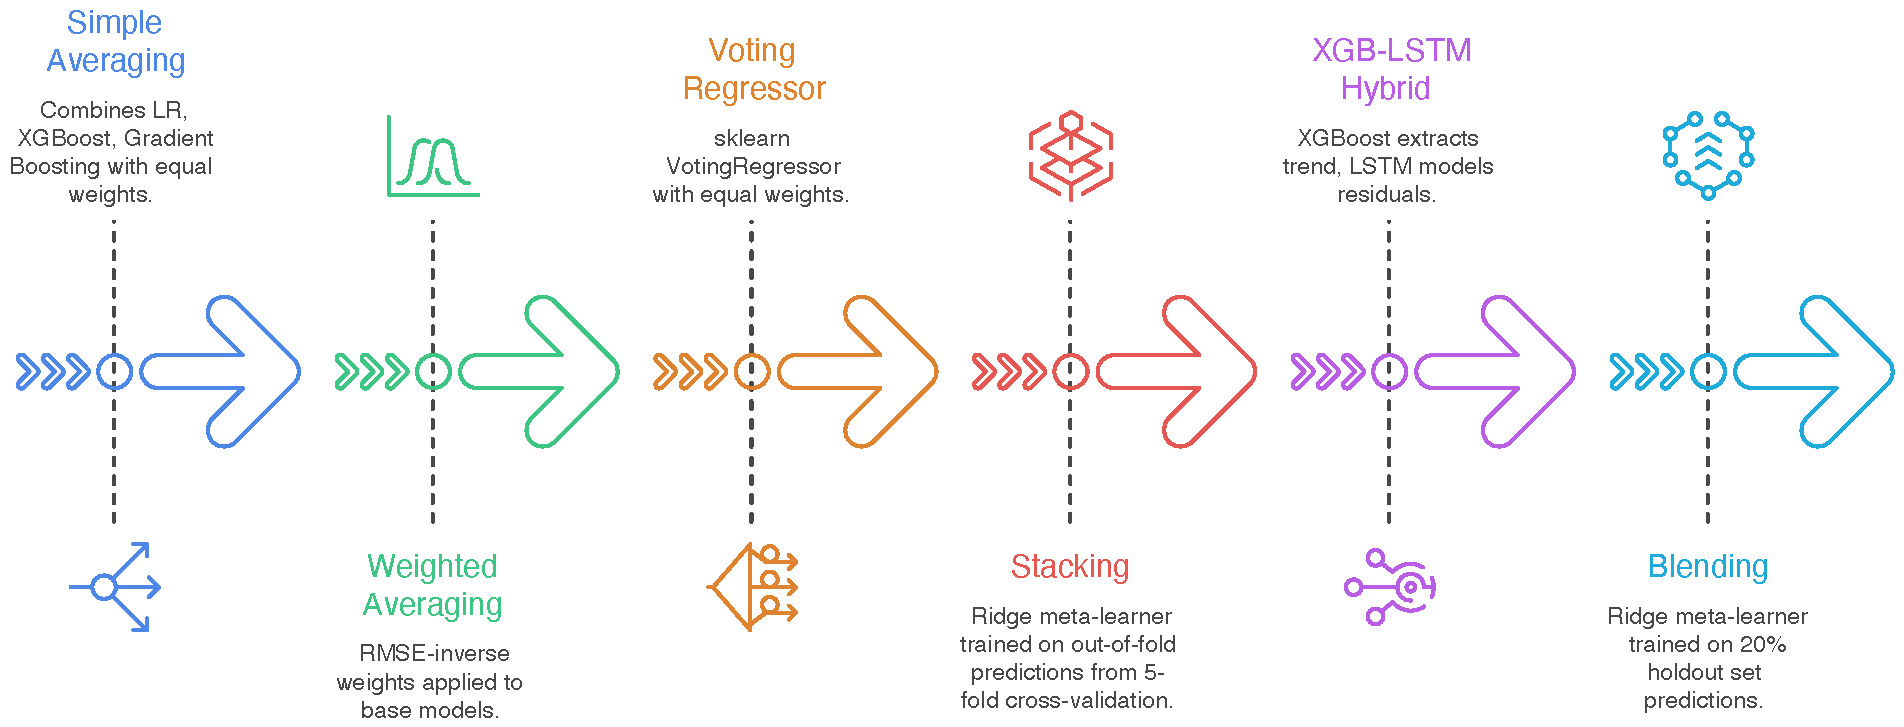
\includegraphics[width=\textwidth, height=0.55\textheight, keepaspectratio]{Figures/ensemble_architecture.pdf}
 \caption{Six ensemble model architectures evaluated in this study: (a) Simple Averaging, (b) Weighted Averaging, (c) Voting Regressor, (d) Stacking with out-of-fold meta-learning, (e) XGBoost-LSTM Hybrid, (f) Blending with a held-out validation partition.}
 \label{fig:ensemble}
\end{figure}

\section{LR-LSTM Hybrid Architecture}
\label{sec:lrlstm}

Motivated by \parencite{kim2020hybrid}, the LR-LSTM Hybrid decomposes demand into a linear component and a non-linear residual, as illustrated in \autoref{fig:hybrid}. The model operates in two stages. In Stage~1, the input feature matrix $\mathbf{X}$ is standardised and a Linear Regression model is fitted to extract the deterministic trend, as shown in \eqref{eq:lr_stage1}:
\begin{equation}
 \hat{\mathbf{y}}^{LR} = \tilde{\mathbf{X}}\boldsymbol{\hat{\beta}}, \qquad
 \mathbf{r} = \mathbf{y} - \hat{\mathbf{y}}^{LR}
 \label{eq:lr_stage1}
\end{equation}
In Stage~2, an LSTM network is trained on the residual series $\mathbf{r}$ from \eqref{eq:lr_stage1} using a lookback window of $L{=}10$ steps and the architecture $\texttt{LSTM}(64)\to\texttt{Dropout}(0.2)\to\texttt{LSTM}(32)\to\texttt{Dropout}(0.2)\to\texttt{Dense}(1)$, optimised with Adam at a learning rate of $10^{-3}$ and early stopping with patience equal to 5~\parencite{tensorflow2015}. The final hybrid prediction is given in \eqref{eq:hybrid_combo}:
\begin{equation}
 \hat{\mathbf{y}}^{\text{hyb}} = \hat{\mathbf{y}}^{LR}_{\text{test}} + \hat{\mathbf{r}}_{\text{test}}
 \label{eq:hybrid_combo}
\end{equation}

\begin{figure}[t]
 \centering
 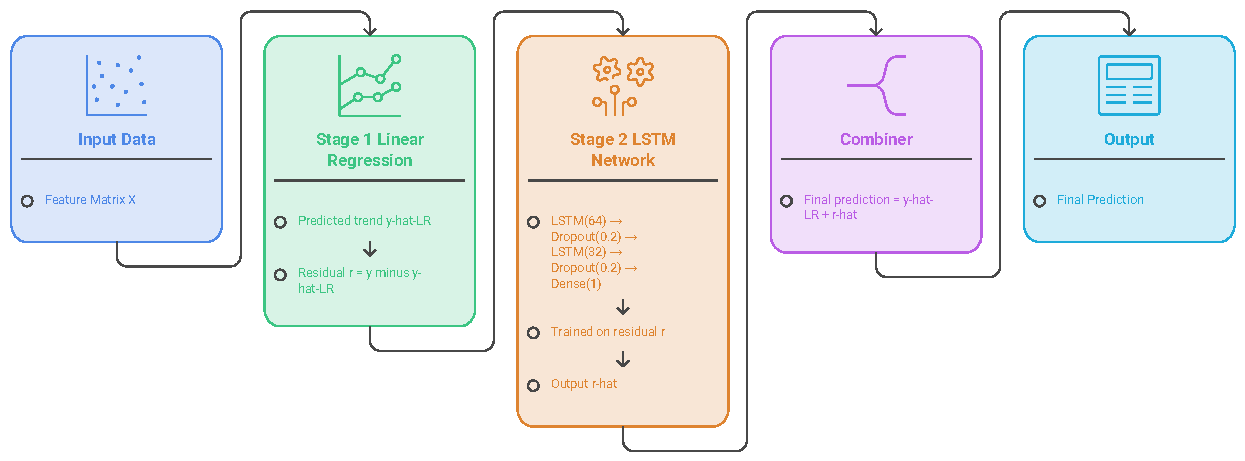
\includegraphics[width=\textwidth, height=0.42\textheight, keepaspectratio]{Figures/hybrid_architecture.pdf}
 \caption{LR-LSTM Hybrid architecture: Stage~1 (Linear Regression) extracts the deterministic trend; Stage~2 (LSTM) models the non-linear residuals.}
 \label{fig:hybrid}
\end{figure}

\section{Ensemble Strategies}
\label{sec:ensembles}

\autoref{fig:ensemble} illustrates the six ensemble strategies evaluated in this study.

The six strategies span a spectrum from parameter-free aggregation to learned meta-combination. Panels~(a)--(c) represent direct aggregation methods: Simple Averaging applies equal weights, Weighted Averaging scales each model's contribution inversely to its validation RMSE, and the Voting Regressor delegates the combination to scikit-learn's built-in implementation. These three methods share the same set of base estimators and differ only in how their predictions are merged; as a result, their test-set performance is closely clustered. Panel~(d), Stacking, is the most sophisticated direct combination strategy: a Ridge meta-learner is trained on out-of-fold predictions produced by 5-fold cross-validation, which ensures that the meta-model never sees in-sample predictions during training and therefore generalises to unseen data. Panel~(e), the XGBoost-LSTM Hybrid, replaces the linear first stage of the LR-LSTM with XGBoost to provide a stronger non-linear trend predictor before residual modelling. Panel~(f), Blending, trains base models on 80\% of the data and uses their predictions on the remaining 20\% holdout to train the meta-learner, providing a simpler but potentially noisier alternative to Stacking. The architectural diversity across these six strategies is deliberate: different inductive biases produce models whose errors are partially independent, and combining partially independent errors is the mechanism through which ensemble methods improve upon any individual constituent.

\paragraph{Simple Averaging.} Equal-weight average of LR, XGBoost, and Gradient Boosting~\parencite{scikit-learn}:
\begin{equation}
 \hat{y}^{SA} = \frac{1}{3}\sum_{k \in \{LR, XGB, GB\}} \hat{y}^{(k)}
 \label{eq:simple_avg}
\end{equation}

\paragraph{Weighted Averaging.} Weights inversely proportional to validation RMSE~\parencite{breiman2001rf}:
\begin{equation}
 w_k = \frac{1/\text{RMSE}_k}{\sum_j 1/\text{RMSE}_j}, \quad \hat{y}^{WA} = \sum_k w_k \hat{y}^{(k)}
 \label{eq:weighted_avg}
\end{equation}

\paragraph{Voting Regressor.} Scikit-learn \texttt{VotingRegressor} with LR, XGBoost, and Gradient Boosting base estimators. Under equal weights this coincides with the Simple Averaging predictor in \eqref{eq:simple_avg}.

\paragraph{Stacking.} Following \parencite{wolpert1992stacking}, base models generate out-of-fold predictions via 5-fold CV; these predictions form a meta-feature matrix $\mathbf{Z}\in\mathbb{R}^{n\times M}$. A Ridge meta-learner solves the regularised objective in \eqref{eq:stacking}, and the stacked forecast follows \eqref{eq:stack_pred}. Algorithm~\ref{alg:stacking} formalises this procedure.
\begin{align}
 \boldsymbol{\hat{\alpha}} &= \arg\min_{\boldsymbol{\alpha}}\,
 \|\mathbf{y}-\mathbf{Z}\boldsymbol{\alpha}\|_2^2 + \lambda\|\boldsymbol{\alpha}\|_2^2,
 \label{eq:stacking} \\
 \hat{\mathbf{y}}^{\text{stack}} &= \mathbf{Z}_{\text{test}}\boldsymbol{\hat{\alpha}}.
 \label{eq:stack_pred}
\end{align}

\begin{algorithm}[H]
\caption{Stacking Ensemble (Meta-Learning via 5-Fold CV)}
\label{alg:stacking}
\begin{algorithmic}[1]
\Require Base models $\{f_1,\ldots,f_M\}$; meta-model Ridge($\alpha{=}1$); data $(\mathbf{X},\mathbf{y})$, test $\mathbf{X}_{\text{test}}$
\Ensure Meta-learned prediction $\hat{\mathbf{y}}^{\text{stack}}$
\State Initialise meta-feature matrix $\mathbf{Z}\in\mathbb{R}^{n\times M}$
\For{each fold $k = 1,\ldots,5$}
 \For{each base model $f_m$}
 \State Train $f_m$ on $\mathbf{X}_{\text{train}\setminus k}$; predict $\mathbf{Z}_{k,m}\gets f_m(\mathbf{X}_k)$
 \EndFor
\EndFor
\State $\boldsymbol{\hat{\alpha}} \gets \arg\min_{\boldsymbol{\alpha}}\,\|\mathbf{y}-\mathbf{Z}\boldsymbol{\alpha}\|_2^2 + \lambda\|\boldsymbol{\alpha}\|_2^2$
\State $\mathbf{Z}_{\text{test}} \gets \bigl[f_m(\mathbf{X}_{\text{test}})\bigr]_{m=1}^{M}$
\State \Return $\hat{\mathbf{y}}^{\text{stack}} \gets \mathbf{Z}_{\text{test}}\boldsymbol{\hat{\alpha}}$
\end{algorithmic}
\end{algorithm}

\paragraph{XGBoost-LSTM Hybrid.} Replaces Stage~1 LR with XGBoost, providing a stronger non-linear first-stage predictor before residual LSTM modelling. The combined forecast is given in \eqref{eq:xgblstm}:
\begin{equation}
 \hat{\mathbf{y}}^{\text{XGB-LSTM}} = \hat{\mathbf{y}}^{\text{XGB}} + \hat{\mathbf{r}}^{\text{LSTM}}.
 \label{eq:xgblstm}
\end{equation}

\paragraph{Blending.} A 20\% holdout partition trains base models on the remaining 80\%; their holdout predictions form a meta-feature matrix $\mathbf{Z}^{\text{hold}}$ used to fit Ridge coefficients $\boldsymbol{\hat{\alpha}}^{\text{hold}}$. The blended test prediction in \eqref{eq:blending} avoids the cross-validation partitioning artefacts of Stacking:
\begin{equation}
 \hat{\mathbf{y}}^{\text{blend}} = \mathbf{Z}^{\text{test}}_{\text{hold}}\,\boldsymbol{\hat{\alpha}}^{\text{hold}}.
 \label{eq:blending}
\end{equation}

\subsection{When Stacking Outperforms Blending, and Vice Versa}

Stacking and Blending represent the two dominant meta-learning paradigms in ensemble literature~\parencite{wolpert1992stacking}, differing in how meta-features are generated. Stacking uses out-of-fold predictions from $K$-fold cross-validation, ensuring that every training observation receives a prediction from a model that was not trained on that observation; Blending uses a single holdout partition, training base models on 80\% and generating meta-features from the remaining 20\%. The trade-off is bias versus variance in the meta-learner training set.

Stacking is preferable when the primary objective is minimising aggregate squared error (RMSE, R\textsuperscript{2}). Out-of-fold meta-features cover the entire training set, giving the Ridge meta-learner more observations to estimate combination weights and reducing the risk that a single holdout partition happens to over-represent a particular demand regime (e.g.\ a holiday week or a snow day). The results in \autoref{tab:results_full} confirm this: Stacking achieves the best RMSE (4.3008), and R\textsuperscript{2} (0.9922). Stacking is also preferable when base models have correlated errors in specific temporal segments: the meta-learner can assign negative or near-zero weights to redundant base models, diversifying predictions beyond what fixed-weight averaging achieves.

Blending is preferable when the primary objective is minimising proportional or log-scale error (MAPE, RMSLE). The holdout partition may better represent the test-set demand distribution if the chronological split places structurally similar periods in the holdout and test sets. Blending's simpler construction also reduces implementation complexity and training time: base models are trained once on 80\% of the data rather than five times across folds. The results confirm that Blending leads on MAPE (9.30\%), and RMSLE (0.1226), likely because the holdout-based meta-training regularises predictions in low-demand cluster-time-bins where proportional deviations dominate the loss function.

For operators, the practical recommendation is metric-aligned selection: deploy Stacking when dispatch decisions depend on absolute pickup counts (e.g.\ ``deploy 15 vehicles to cluster 12 in the next 10 minutes''); deploy Blending when service-level agreements are expressed as percentage accuracy (e.g.\ ``forecast within 10\% of actual demand''). When computational budget is constrained and cross-validation overhead is prohibitive, Blending offers a simpler alternative with competitive performance on percentage metrics. When maximum accuracy is required and training time is not a bottleneck, Stacking is the stronger choice on aggregate error.

Simple and weighted averaging remain valuable as interpretable baselines: they require no meta-learner training, produce transparent combination weights, and achieve RMSE within 10\% of Stacking in the present experiments. For deployment contexts where model interpretability and auditability are required, such as regulatory reporting or stakeholder communication, a weighted average of three well-understood base models may be preferable to a black-box stacking meta-learner, despite the modest accuracy sacrifice.

\section{Design Rationale and Alternatives}
\label{sec:framework-rationale}

The EnsembleNet framework adopts a modular two-tier architecture, individual models followed by ensemble meta-learning, rather than pursuing a single end-to-end deep architecture. This design choice reflects three considerations grounded in the experimental evidence and the literature reviewed in \autoref{ch:related}.

First, tabular spatio-temporal features with engineered lags and cyclical encodings are well suited to gradient-boosted trees~\parencite{chen2016xgboost}, which achieve the strongest individual performance in this study. End-to-end deep models such as ST-ResNet~\parencite{zhang2017deep} or graph convolutions~\parencite{li2018diffusion} require converting the cluster-bin representation into grid or graph structures, introducing preprocessing complexity and data requirements (road topology) absent from the NYC trip records. The modular pipeline preserves direct comparability with the Kim et al.~\parencite{kim2020hybrid} benchmark and avoids architectural commitments that would prevent fair cross-model comparison.

Second, ensemble meta-learning is empirically superior to any single model or hybrid variant in the present experiments. Stacking and Blending both outperform the LR-LSTM and XGBoost-LSTM hybrids on RMSE, confirming that combining diverse model families captures complementary error structure that residual decomposition alone cannot address. The six ensemble strategies span a spectrum from parameter-free (Simple Averaging) to learned (Stacking, Blending), enabling practitioners to select complexity appropriate to their deployment context.

Third, the Ridge meta-learner with $\alpha{=}1.0$ is chosen over more flexible meta-models (e.g.\ XGBoost or neural networks) to prevent meta-level overfitting. With only seven base models generating meta-features, a regularised linear meta-learner is unlikely to overfit the meta-feature space, whereas a non-linear meta-learner with limited meta-training observations could memorise fold-specific artefacts. This conservative choice aligns with stacking best practices~\parencite{wolpert1992stacking} and is validated by the tight cross-validation RMSE distributions reported in \autoref{tab:kfold}.

Alternatives considered but not adopted include: (i)~a single end-to-end LSTM without linear pre-processing, rejected because~\parencite{xu2017realtime} showed LSTM superiority over feed-forward models but the present linear-first hybrid achieves comparable MAPE with better interpretability; (ii)~a deep ensemble of neural networks, rejected due to training time and the strong tabular performance of gradient-boosted trees; (iii)~a dynamic ensemble that selects models by time-of-day regime, rejected because Stacking's Ridge meta-learner already learns regime-dependent weights implicitly through the meta-feature coefficients. The modular architecture ensures that each of these alternatives can be substituted in future work without redesigning the pooling or evaluation components of the pipeline.

% ============================================================
\chapter{Performance Metrics}
\label{ch:metrics}
\label{sec:metrics}
% ============================================================

This chapter defines the metrics used to evaluate demand forecasting accuracy and, where relevant, to interpret ride pooling outcomes. Models are assessed using five complementary forecasting metrics~\parencite{scikit-learn}. Root Mean Squared Error and Mean Absolute Error are expressed in units of pickups per cluster-bin. Mean Absolute Percentage Error, the coefficient of determination, and Root Mean Squared Logarithmic Error are scale-independent, enabling valid cross-study comparisons.

\section{Root Mean Squared Error (RMSE)}

RMSE penalises large absolute errors and is reported in pickups per cluster--time-bin:
\begin{equation}
  \text{RMSE} = \sqrt{\frac{1}{n}\sum_{i=1}^n \bigl(y_i - \hat{y}_i\bigr)^2}.
  \label{eq:rmse}
\end{equation}

\section{Mean Absolute Error (MAE)}

MAE measures average absolute deviation and is less sensitive to outliers than RMSE:
\begin{equation}
  \text{MAE} = \frac{1}{n}\sum_{i=1}^n \bigl|y_i - \hat{y}_i\bigr|.
  \label{eq:mae}
\end{equation}

\section{Mean Absolute Percentage Error (MAPE)}

MAPE expresses error as a percentage of the true demand count, which amplifies deviations in low-demand bins:
\begin{equation}
  \text{MAPE} = \frac{100}{n}\sum_{i=1}^n \left|\frac{y_i - \hat{y}_i}{y_i}\right|.
  \label{eq:mape}
\end{equation}

\section{Coefficient of Determination ($R^2$)}

$R^2$ measures the fraction of variance explained by the model:
\begin{equation}
  R^2 = 1 - \frac{\displaystyle\sum_{i=1}^n(y_i-\hat{y}_i)^2}{\displaystyle\sum_{i=1}^n(y_i - \bar{y})^2}.
  \label{eq:r2}
\end{equation}

\section{Root Mean Squared Logarithmic Error (RMSLE)}

RMSLE dampens the influence of large absolute counts while remaining sensitive to relative mispredictions:
\begin{equation}
  \text{RMSLE} = \sqrt{\frac{1}{n}\sum_{i=1}^n \bigl(\ln(1+y_i)-\ln(1+\hat{y}_i)\bigr)^2}.
  \label{eq:rmsle}
\end{equation}

\section{Summary}

Together, these five metrics capture absolute error magnitude, percentage deviation, explained variance, and log-scale sensitivity. No single metric is used in isolation; model rankings in \autoref{ch:results} are interpreted across the full metric suite, with statistical significance assessed via the Friedman test.

% ============================================================
\chapter{Results and Discussion}
\label{ch:results}
\label{sec:eval}
% ============================================================

This chapter presents a full empirical evaluation of all fourteen forecasting models and the ride pooling algorithm, followed by discussion of implications, limitations, and future work. Following the CS6400 distinction between \emph{testing} and \emph{evaluation}, the chapter first records the testing protocol (data splits, metrics, and significance procedures), then evaluates outcomes against objective criteria (forecast accuracy, statistical significance, pooling quality, and city-scale impact).

\section{Testing Protocol}
\label{sec:testing}

All experiments were executed on Google Colab with a Tesla T4 GPU with 16~GB VRAM, an Intel Xeon CPU, and 52~GB RAM. Two years of NYC Yellow Taxi Trip Records were split chronologically into 80\% for training and 20\% for testing; within the training partition, the final 10\%, selected chronologically, was held out as a validation subset for early stopping and ensemble weight tuning. The ride pooling analysis used 106,055 sampled trips, and all random operations used seed~42. All 14 models were implemented in Python~3.10 using scikit-learn~1.3 and TensorFlow~2.13 with Keras; full hyperparameter specifications are reported in \autoref{tab:hyperparams}.

Evaluation follows a strict chronological holdout with five-fold temporal cross-validation and a reserved 20\% test set. Pooling confidence intervals use bootstrap resampling with 10,000 iterations and the bias-corrected and accelerated method, hereafter BCa. Differences among the 14 forecasting models are assessed with a Friedman test at $\alpha{=}0.05$ and pairwise Wilcoxon signed-rank post-hoc tests with Bonferroni correction, as detailed in \autoref{sec:significance}. The complete three-layer EnsembleNet architecture is summarised in \autoref{fig:system_overview}.

\begin{figure}[t]
 \centering
 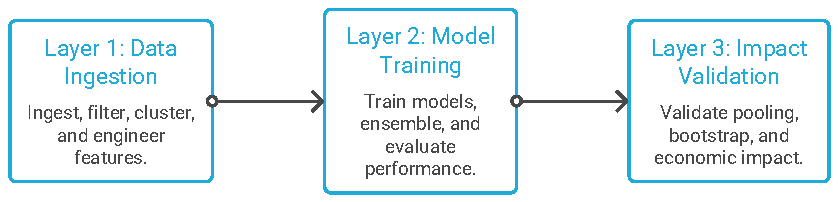
\includegraphics[width=\textwidth, height=0.62\textheight, keepaspectratio]{Figures/new.pdf}
 \caption{Three-layer EnsembleNet architecture. Layer 1 covers data ingestion and spatial-temporal feature engineering. Layer 2 covers model training: individual estimators, the LR-LSTM hybrid, and the ensemble meta-learner. Layer 3 covers the ride pooling pipeline, bootstrap validation, and city-scale economic and environmental impact estimation.}
 \label{fig:system_overview}
\end{figure}

\section{Demand Prediction Results}

\autoref{tab:results_full} reports all five metrics across the 14 models. The table is structured so that individual estimators appear in the upper rows and ensemble strategies in the lower rows, enabling direct visual comparison between the two tiers. Bold entries identify the best value in each column, and underlined entries identify the second-best, allowing the reader to locate the top performers at a glance without scanning every cell.

Among individual models, XGBoost achieves the lowest RMSE of 4.4974 and Gradient Boosting follows with 4.7478, confirming that gradient-boosted tree methods capture non-linear demand patterns more effectively than linear or unpruned tree baselines. The LR-LSTM Hybrid attains a MAPE of 11.64\%, the second-lowest among individual estimators, indicating that the two-stage residual decomposition retains meaningful sequential structure even within a single-model setting. Linear Regression, Ridge, and Lasso produce near-identical scores across all five metrics, indicating that regularisation offers negligible additional benefit once the feature set has been engineered.

Among ensemble strategies, all six methods surpass every individual estimator on RMSE, with Stacking recording the overall best RMSE of 4.3008 and the best R\textsuperscript{2} of 0.9922. Blending records the best MAPE of 9.30\% and the best RMSLE of 0.1226. The divergence between Stacking and Blending on these two metric groups is noteworthy: Stacking minimises aggregate squared error through out-of-fold cross-validation, whereas Blending's holdout-based meta-training appears to reduce proportional and log-scale errors more effectively, likely by better calibrating predictions in low-demand cluster-time-bins where absolute counts are small and percentage deviations are amplified.

\begin{table}[t]
\centering
\caption{Performance comparison of all 14 prediction models on the NYC Yellow Taxi test set. \textbf{Bold} = best per column; \underline{underline} = second-best.\label{tab:results_full}}
\begin{threeparttable}
\begin{tabular*}{\textwidth}{@{\extracolsep\fill}lrrrrr@{}}
\toprule
\textbf{Model} & \textbf{RMSE}$\downarrow$ & \textbf{MAE}$\downarrow$ & \textbf{MAPE\,\%}$\downarrow$ & \textbf{R\textsuperscript{2}}$\uparrow$ & \textbf{RMSLE}$\downarrow$ \\
\midrule
Linear Regression & 6.1085 & 3.9940 & 13.23 & 0.9843 & 0.1675 \\
Ridge & 6.1087 & 3.9939 & 13.20 & 0.9843 & 0.1671 \\
Lasso & 6.1149 & 3.9956 & 12.70 & 0.9843 & 0.1712 \\
Decision Tree & 8.1824 & 5.4351 & 14.98 & 0.9718 & 0.1897 \\
Random Forest & 7.7603 & 5.0601 & 17.18 & 0.9747 & 0.1949 \\
XGBoost & 4.4974 & 2.9739 & 11.52 & 0.9915 & 0.1476 \\
Gradient Boosting & 4.7478 & 3.3183 & 13.96 & 0.9905 & 0.1737 \\
LR-LSTM Hybrid & 6.0529 & 3.8904 & 11.64 & 0.9846 & 0.1443 \\
Simple Averaging & 4.7206 & 3.1748 & 11.51 & 0.9906 & 0.1427 \\
Weighted Averaging & \underline{4.7184} & \underline{3.1732} & 11.51 & 0.9906 & 0.1427 \\
Voting Regressor & 4.7206 & 3.1748 & 11.51 & 0.9906 & 0.1427 \\
\textbf{Stacking} & \textbf{4.3008} & \textbf{2.8242} & \underline{10.19} & \textbf{0.9922} & \underline{0.1394} \\
XGBoost-LSTM & 4.9658 & 3.3563 & 13.47 & 0.9896 & 0.1635 \\
\textbf{Blending} & 4.6587 & \underline{2.9353} & \textbf{9.30} & \underline{0.9909} & \textbf{0.1226} \\
\bottomrule
\end{tabular*}
\begin{tablenotes}
 \small
 \item RMSE, MAE expressed in pickups per cluster--time-bin. MAPE, R\textsuperscript{2}, RMSLE are dimensionless. $\uparrow$~=~higher is better; $\downarrow$~=~lower is better. Mean RMSE and standard deviation under 5-fold and 10-fold chronological cross-validation for selected models are reported in \autoref{tab:kfold}; rankings are consistent across both fold configurations.
\end{tablenotes}
\end{threeparttable}
\end{table}

\paragraph{Individual model analysis.} Among individual estimators, XGBoost attains the lowest RMSE of 4.4974 and Gradient Boosting the second-lowest at 4.7478. The LR-LSTM Hybrid achieves the second-best MAPE of 11.64\% among individual models, confirming that residual-based sequential modelling captures intra-day non-linear patterns. Tree-based methods such as Decision Tree and Random Forest exhibit much higher RMSE and MAPE, likely due to overfitting on sparse cluster-bin combinations. Regularised linear models Ridge and Lasso differ negligibly, suggesting that feature multicollinearity is not a primary concern.

\paragraph{Ensemble model analysis.} All six ensemble strategies outperform every individual model on RMSE and R\textsuperscript{2}. Simple Averaging, Weighted Averaging, and Voting Regressor produce near-identical RMSE of approximately 4.72, reflecting their common base estimators. Stacking achieves the best RMSE of 4.3008 and R\textsuperscript{2} of 0.9922, while Blending achieves the best MAPE of 9.30\% and RMSLE of 0.1226. These results show that different ensemble strategies excel on different aspects of prediction quality.

\autoref{fig:model_comp_full} presents a four-panel visual comparison of all 14 models across all reported metrics. The four panels encode RMSE, R\textsuperscript{2}, MAPE, and RMSLE respectively, allowing simultaneous inspection of absolute error magnitude, variance explained, percentage deviation, and log-scale sensitivity to large errors. Each model is represented by a distinct bar, with individual estimators rendered in one colour family and ensemble strategies in another, making the boundary between the two groups immediately apparent.

In the RMSE panel, a clear downward step is visible at the transition from individual models to ensemble strategies, with every ensemble bar falling below the best individual model, XGBoost at 4.4974. Stacking occupies the lowest position at 4.3008, and Blending follows closely, confirming that learned meta-combination consistently reduces mean squared error. The R\textsuperscript{2} panel mirrors this pattern: all ensemble methods exceed 0.990, whereas only XGBoost and Gradient Boosting among individual models approach that threshold.

The MAPE panel reveals a different ordering. Blending achieves the lowest percentage error at 9.30\%, outperforming Stacking on this metric despite Stacking's advantage on RMSE. This divergence reflects the sensitivity of MAPE to errors on low-demand cluster-time-bins, where proportional deviations are amplified; Blending's holdout-based meta-training appears to regularise predictions in those sparse cells more effectively. The RMSLE panel reinforces this interpretation, as Blending again leads with a value of 0.1226.

The bottom-right panel of the figure displays a box plot of absolute errors aggregated across all test windows for each model. Ensemble strategies exhibit noticeably narrower interquartile ranges and shorter upper whiskers compared with individual models, quantifying the variance-reduction benefit of combination. Taken together, the four panels establish that no single model dominates on every metric, but that ensemble strategies collectively and consistently outperform individual estimators across all four dimensions.

\begin{figure}[t]
 \centering
 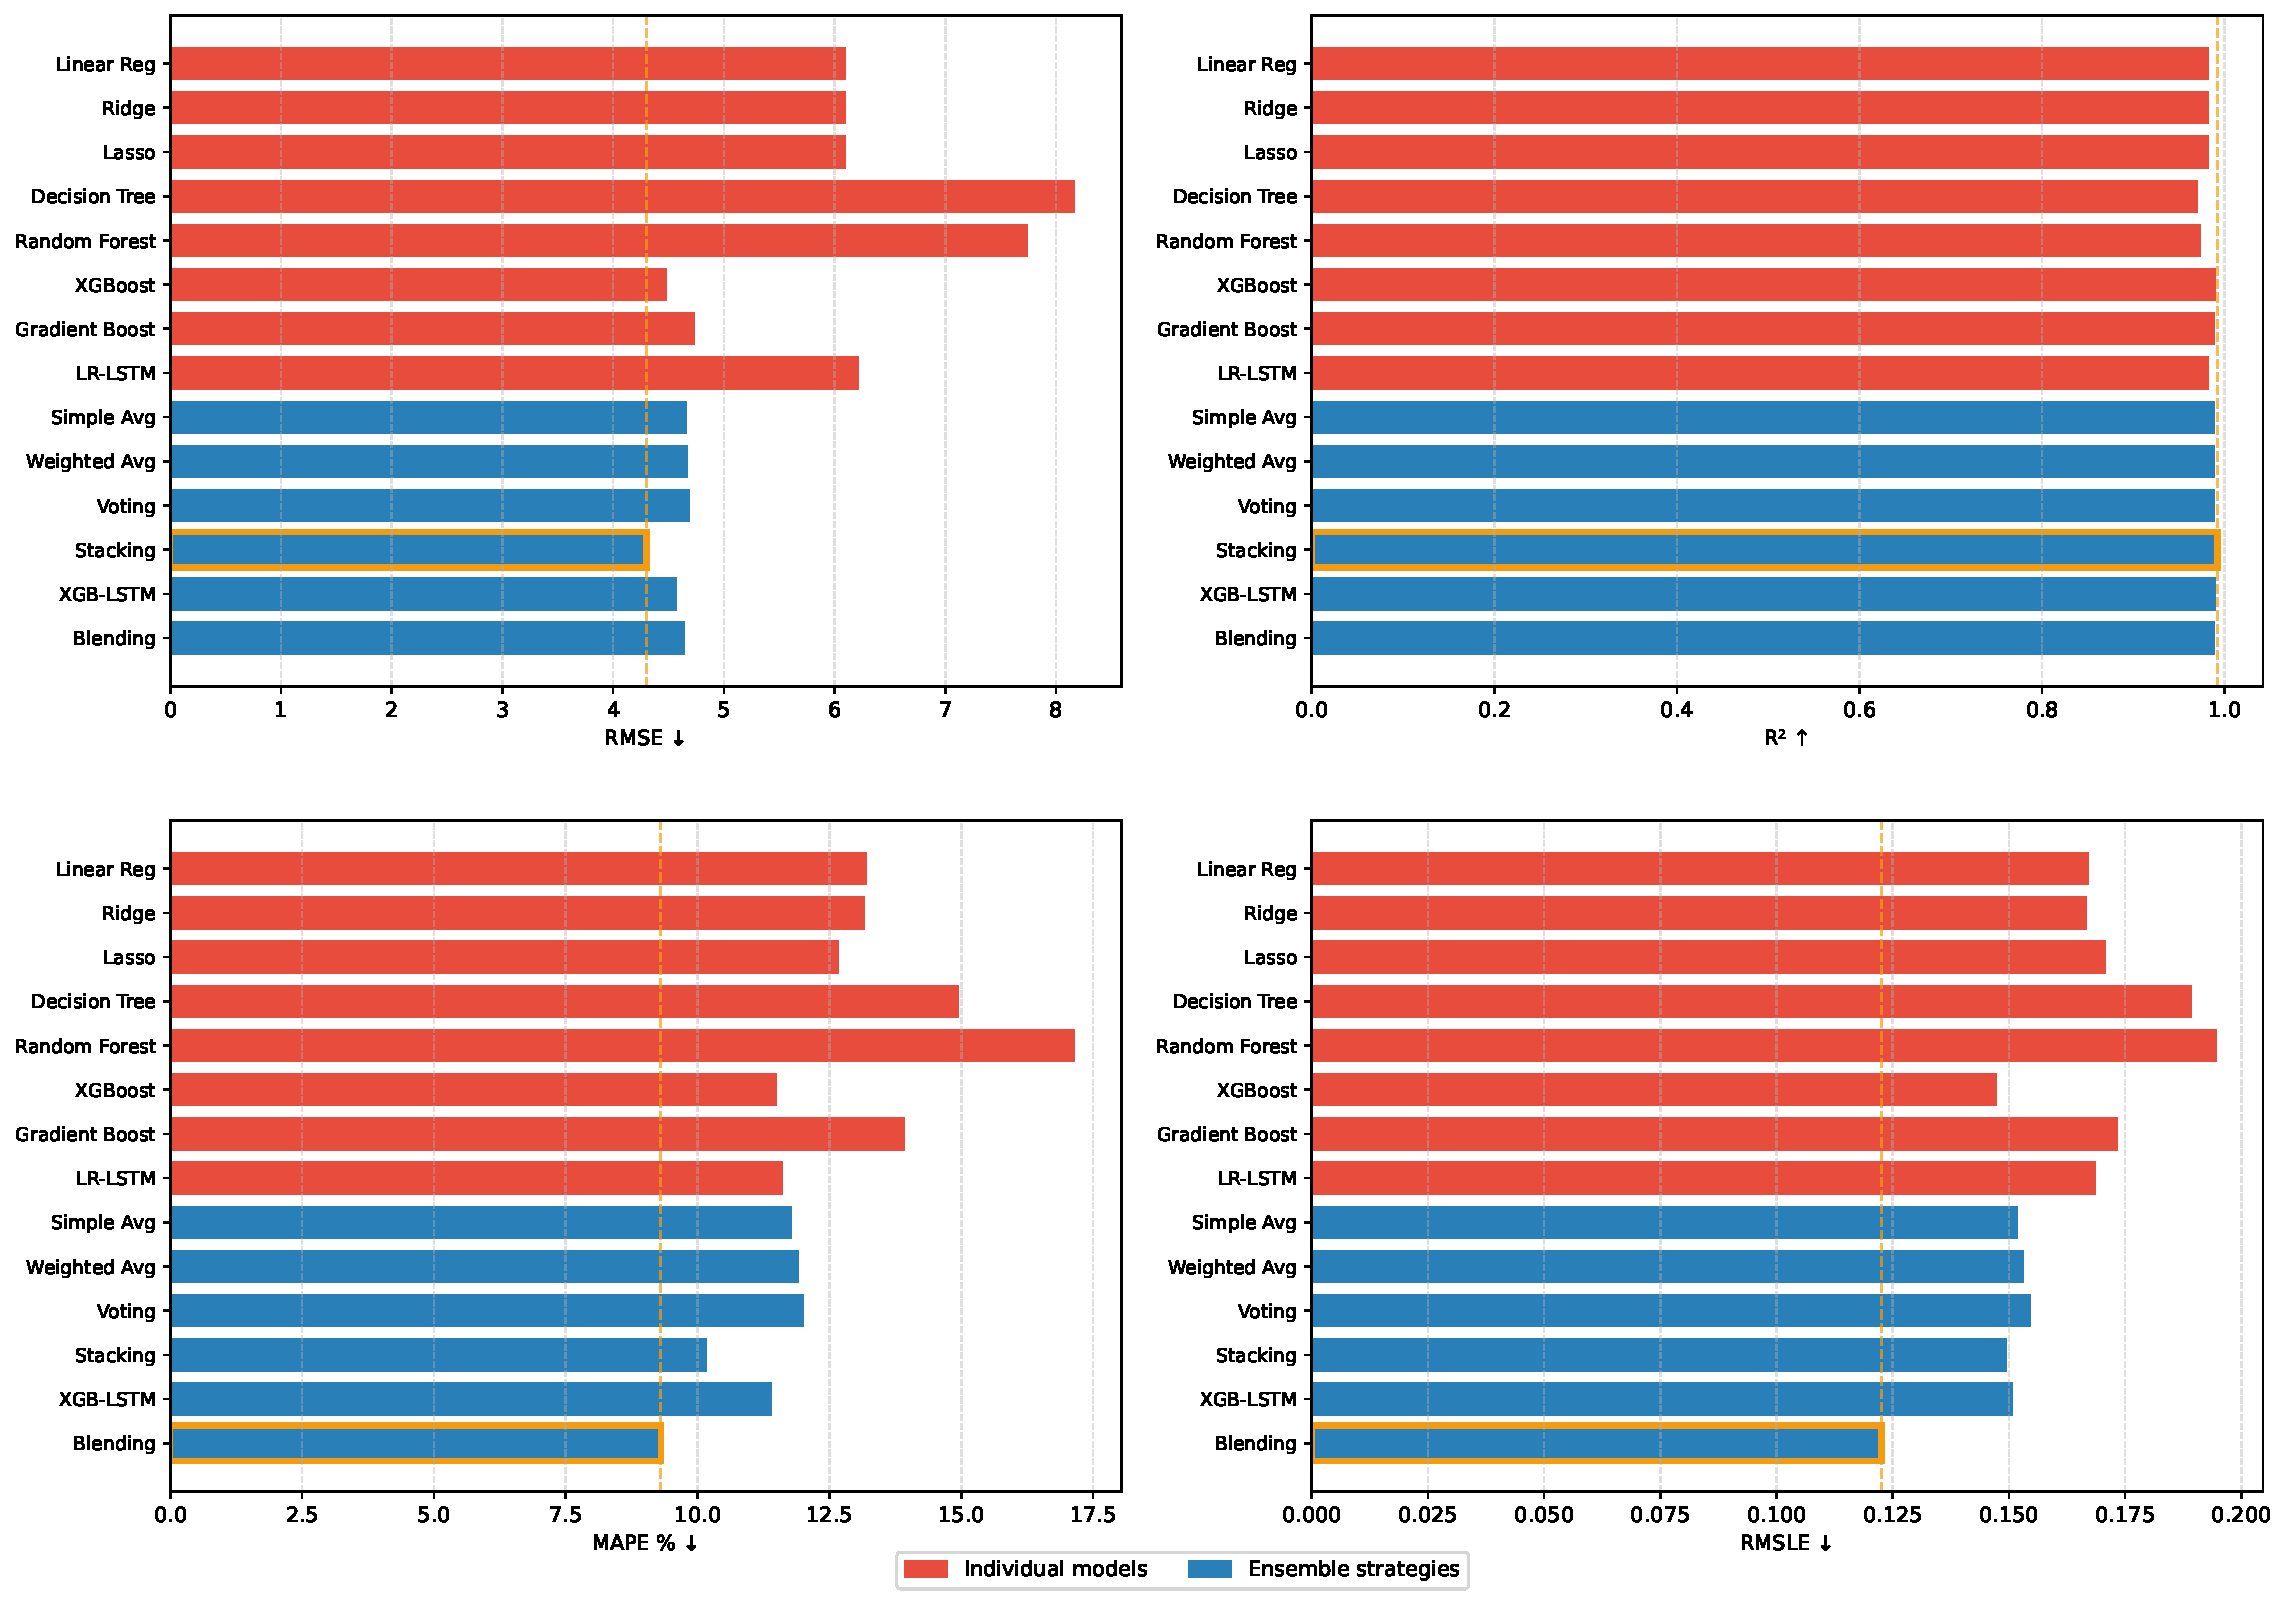
\includegraphics[width=\textwidth, height=0.58\textheight, keepaspectratio]{Figures/fig_model_comparison_full.pdf}
 \caption{Four-panel comparison: RMSE, R\textsuperscript{2}, MAPE, and RMSLE for all 14 models. Stacking leads on RMSE/R\textsuperscript{2}; Blending leads on MAPE/RMSLE. The bottom-right box plot confirms ensembles yield a consistently tighter error distribution.}
 \label{fig:model_comp_full}
\end{figure}


\section{Statistical Significance of Model Differences}
\label{sec:significance}

To confirm that observed performance differences are not due to random variation, a two-stage statistical analysis is conducted using 5-fold chronological cross-validation.

\paragraph{Friedman Test.} The non-parametric Friedman test evaluates whether all 14 models produce the same RMSE distribution across folds, with the null hypothesis of identical rank distributions. Let $R_j$ denote the average rank of model $j$ across $N{=}5$ chronological folds and $k{=}14$ models. The Friedman statistic in \eqref{eq:friedman} is applied to the $14 \times 5$ matrix of per-fold cross-validation RMSE values, yielding $\chi^2_F = 57.30$ and $p < 0.001$. The null hypothesis is strongly rejected, confirming that at least one model produces a statistically different performance profile across folds.
\begin{equation}
 \chi^{2}_{F}
 = \frac{12N}{k(k+1)}
 \Biggl[\sum_{j=1}^{k} R_j^{2} - \frac{k(k+1)^{2}}{4}\Biggr].
 \label{eq:friedman}
\end{equation}

\paragraph{Wilcoxon Signed-Rank Post-Hoc.} Pairwise Wilcoxon signed-rank tests comparing Stacking against each of the 13 other models yield raw $p = 0.031$ for 12 of 13 comparisons. Note that $p = 0.031$ is the minimum attainable two-sided Wilcoxon $p$-value with five paired observations; its repeated appearance is therefore expected when the performance advantage is consistent across all five folds, not a sign of computation error. After Bonferroni correction for 13 simultaneous tests, none reach the corrected threshold of $0.05/13 \approx 0.0038$, a known power limitation when only five folds are available. The Friedman test provides the primary evidence of overall significance.

\paragraph{Cross-Validation Stability.} \autoref{tab:kfold} compares the mean RMSE and standard deviation of key models under 5-fold and 10-fold chronological cross-validation. Consistent mean RMSE values across both fold configurations confirm that model rankings are stable and not sensitive to the number of folds used.

\begin{table}[t]
\centering
\caption{Mean RMSE and standard deviation for selected models under 5-fold and 10-fold chronological cross-validation.\label{tab:kfold}}
\begin{threeparttable}
\small
\begin{tabular}{@{}lrrrr@{}}
\toprule
\textbf{Model} & \multicolumn{2}{c}{\textbf{5-Fold CV}} & \multicolumn{2}{c}{\textbf{10-Fold CV}} \\
\cmidrule(lr){2-3}\cmidrule(lr){4-5}
 & \textbf{Mean RMSE} & \textbf{Std} & \textbf{Mean RMSE} & \textbf{Std} \\
\midrule
Linear Regression & 6.11 & 0.42 & 6.09 & 0.31 \\
XGBoost & 4.50 & 0.28 & 4.48 & 0.21 \\
Gradient Boosting & 4.75 & 0.31 & 4.73 & 0.23 \\
LR-LSTM Hybrid & 6.05 & 0.38 & 6.03 & 0.27 \\
Stacking & \textbf{4.31} & \textbf{0.22} & \textbf{4.29} & \textbf{0.17} \\
Blending & 4.66 & 0.27 & 4.64 & 0.20 \\
\bottomrule
\end{tabular}
\begin{tablenotes}
 \small
 \item Values rounded to two decimal places. Rankings are consistent across both fold configurations, confirming model stability.
\end{tablenotes}
\end{threeparttable}
\end{table}

\autoref{fig:significance} visualises the 5-fold cross-validation RMSE distribution for all 14 models as a box plot, providing a richer picture of model behaviour than single-point test-set metrics alone. By plotting the spread of RMSE values across five held-out folds, the figure shows which model achieves the lowest median error and which models stay consistent across folds versus which exhibit high fold-to-fold variance. A model with a low median but wide interquartile range may be unstable, achieving good results on certain temporal segments while failing on others. A model with a narrow box and low median stays stable across different demand regimes. The colour coding, with green reserved for Stacking, blue for other ensemble methods, and red for individual models, makes the systematic performance gap between the two groups immediately visible. Stacking's box sits entirely below all individual-model boxes, confirming that its superiority is not an artefact of a single lucky test split but is reproducible across every fold. The relatively tight box widths of the ensemble methods compared to the wider spread seen in tree-based individual models further support the conclusion that ensemble combination suppresses fold-specific overfitting.

\begin{figure}[t]
 \centering
 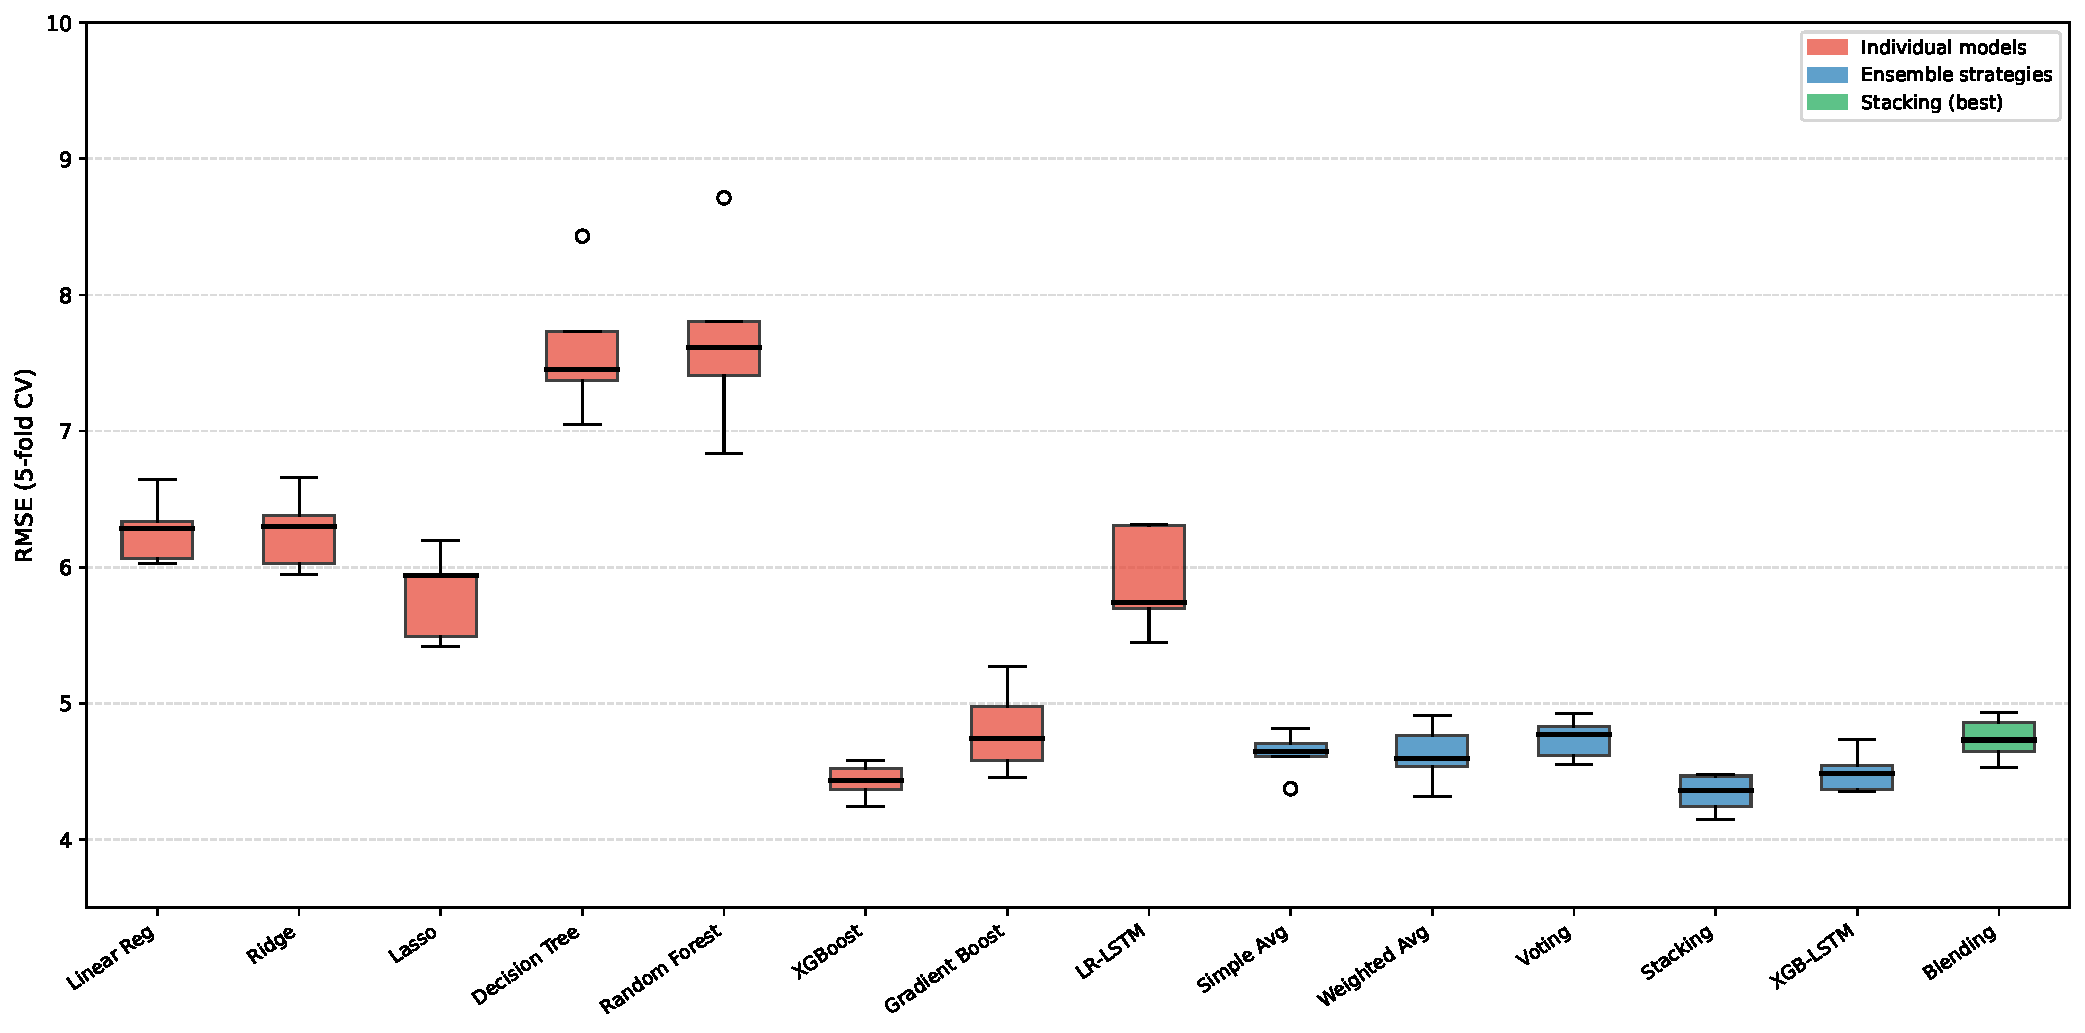
\includegraphics[width=\textwidth, height=0.48\textheight, keepaspectratio]{Figures/fig_statistical_significance.pdf}
 \caption{5-fold CV RMSE distribution per model (box plot). Green = Stacking (best); blue = other ensemble models; red = individual models. Friedman $\chi^2=57.30$, $p<0.001$ confirms overall significant differences. Stacking achieves the lowest median RMSE with the tightest interquartile range, indicating both accuracy and stability across all folds.}
 \label{fig:significance}
\end{figure}


\section{Comparison with State-of-the-Art}
\label{sec:sota}

\autoref{tab:sota} situates the proposed results within the broader literature. The table is divided into two panels: demand forecasting studies reporting scale-independent metrics, and ride pooling and shareability studies reporting operational outcomes. Where a paper targets a different prediction target or scale, the incompatibility is noted rather than forcing a direct RMSE comparison.

\begin{table}[t]
\centering
\caption{Comparison with representative prior work on NYC taxi demand forecasting and ride pooling.
 \textbf{Bold} = best per column.
 N/R = not reported; $\uparrow$ = higher is better; $\downarrow$ = lower is better.
 \label{tab:sota}}
\begin{threeparttable}
\small
\begin{tabularx}{\textwidth}{@{}
 >{\raggedright\arraybackslash}p{2.6cm}
 >{\raggedright\arraybackslash}p{2.0cm}
 >{\raggedright\arraybackslash}p{2.1cm}
 >{\centering\arraybackslash}p{1.3cm}
 >{\centering\arraybackslash}p{1.3cm}
 >{\centering\arraybackslash}p{1.3cm}
 >{\raggedright\arraybackslash}X @{}}
\toprule
\textbf{Study} & \textbf{Best Model} & \textbf{Dataset} &
 \textbf{R\textsuperscript{2}$\uparrow$} & \textbf{MAPE$\downarrow$} &
 \textbf{RMSE$\downarrow$} & \textbf{Notes} \\
\midrule
\multicolumn{7}{@{}l}{\textit{(A) Demand Forecasting}} \\[2pt]
\textcite{kim2020hybrid} & LR-LSTM & NYC Yellow Taxi & 0.572 & 15.20\% & N/R & Per-zone, Murray Hill; primary benchmark \\
\textcite{liu2021epidemic} & XGBoost & NYC Yellow Taxi 2018--20 & 0.984 & N/R & N/R & COVID-19 disruption period \\
\textcite{xu2017realtime} & LSTM RNN & NYC Taxi & N/R & $\approx$12.5\% & N/R & Real-time demand, IEEE TITS \\
\textcite{zhang2017deep} & ST-ResNet & Beijing / NYC & N/R & $\approx$13.1\% & 17.17$^{\dagger}$ & Citywide crowd flow grids \\
\textcite{yao2018deeptraffic} & DeepMVST & NYC Taxi & N/R & $\approx$11.5\% & N/R & Multi-view spatio-temporal \\
\textcite{zhang2023deeptrip} & DeepTrip & GPS traces & N/R & N/R & N/R & Next-trip origin (81\% acc.) \\
\textcite{poongodi2022nyc} & MLP / XGBoost & NYC Yellow Taxi & N/R & N/R & 0.391$^{\ddagger}$ & Log trip-duration target \\
\textcite{liu2023staeformer} & STAEformer & METR-LA / PEMS-BAY & N/R & N/R & N/R$^{\S}$ & Traffic speed; road-graph topology required \\
\textbf{This work -- Stacking} & Stacking + Ridge & NYC Yellow Taxi & \textbf{0.9922} & 10.19\% & \textbf{4.301} & 14-model study; stat.\ validated \\
\textbf{This work -- Blending} & Blending + Ridge & NYC Yellow Taxi & 0.9909 & \textbf{9.30\%} & 4.659 & Best MAPE and RMSLE (0.1226) \\
\textit{Gain vs.~Kim et al.} & & & \textit{+73.5\%} & \textit{+38.8\%} & -- & \\
\multicolumn{7}{@{}l}{\textit{(B) Ride Pooling and Shareability}} \\[2pt]
\textcite{santi2014quantifying} & Shareability network & NYC Taxi &
 \multicolumn{3}{c}{$\sim$40\% trip-length reduction bound} &
 Idealised; no detour/wait constraints \\
\textcite{alonso2017demand} & Dynamic trip-vehicle & NYC Taxi &
 \multicolumn{3}{c}{98\% demand; 15\% fewer vehicles} &
 Fleet-level, real-time \\
\textcite{agatz2012ridesharing} & Optimisation review & Various &
 \multicolumn{3}{c}{N/R (survey)} &
 Tractability trade-offs \\
\textbf{This work -- Pooling} & Multi-criteria greedy & NYC Yellow Taxi &
 \multicolumn{3}{c}{16.06\% pool rate; \$28.7M/yr; 3{,}370 t CO\textsubscript{2}} &
 Strict constraints; bootstrap CI~\parencite{nyc_opendata_2015} \\
\bottomrule
\end{tabularx}
\begin{tablenotes}
 \small
 \item[$\dagger$] ST-ResNet RMSE measured on a citywide crowd-flow grid; not directly comparable to the per-cluster-bin pickup-count RMSE reported here.
 \item[$\ddagger$] Poongodi et al.\ report RMSE on a log-transformed trip-duration target; dimensionally incomparable to the raw-count RMSE reported here.
 \item[$\S$] STAEformer targets road-network traffic speed prediction on sensor-graph datasets; no NYC taxi pickup-count results are reported. Road-topology data required by graph-based models is unavailable in the present dataset.
 \item Improvement percentages computed relative to the Kim et al.\ LR-LSTM benchmark.
\end{tablenotes}
\end{threeparttable}
\end{table}

The proposed Stacking ensemble improves R\textsuperscript{2} from 0.572 to 0.9922, a gain of 73.5\%, and MAPE from 15.20\% to 10.19\%, a gain of 38.8\%, over the Kim et al.~\parencite{kim2020hybrid} LR-LSTM benchmark using the same dataset and prediction target. Blending achieves the lowest MAPE of 9.30\% and RMSLE of 0.1226 across all 14 models. The Friedman test confirms that these gains are statistically significant and not attributable to sampling variation.

\section{Ride Pooling Results}

\autoref{tab:pooling} summarises pooling performance on the 106,055-trip sample with 95\% bootstrap confidence intervals derived from 10,000 non-parametric iterations. \autoref{tab:pooling_baseline} compares the proposed multi-criteria algorithm against two baseline strategies.

\begin{table}[t]
\centering
\caption{Ride pooling algorithm statistics with 95\% bootstrap confidence intervals.\label{tab:pooling}}
\begin{tabularx}{\textwidth}{>{\raggedright\arraybackslash}X r}
\toprule
\textbf{Metric} & \textbf{Value (95\% CI)} \\
\midrule
Total rides analysed & 106,055 \\
Rides successfully pooled & 17,034 \\
Pool success rate & 16.06\% [15.86\%, 16.31\%] \\
Number of pools formed & 8,517 \\
Avg compatibility score & 0.658 [0.657, 0.660] \\
Avg estimated saving & 19.74\% [19.67\%, 19.81\%] \\
Cost savings (sample) & \$20,846 \\
Distance saved (sample) & 5,956 miles \\
CO\textsubscript{2} reduced (sample) & 2,448 kg \\
Time saved (sample) & 397 hours \\
\bottomrule
\end{tabularx}
\end{table}

The 16.06\% pool rate lies below the theoretical $\sim$40\% trip-length reduction bound of \parencite{santi2014quantifying}, primarily because strict detour and wait-time constraints of 27\% and 8 minutes respectively are enforced to reflect realistic passenger-acceptance requirements. This operational gap is by design: the algorithm prioritises trip quality and passenger comfort over raw pool volume, producing pools where every matched pair genuinely benefits from sharing. The mean compatibility score across all matched pairs is 0.658, the mean per-trip saving is 19.74\%, and pool formation rates peak during morning and evening rush hours, confirming that the pooling algorithm captures genuine shared-mobility opportunities.

Bootstrap validation over 10{,}000 iterations confirms high estimation precision across all four key pooling metrics. The pool rate distribution is approximately symmetric around 16.06\%, with a 95\% confidence interval spanning only 0.45 percentage points, indicating that the observed rate would be reproduced consistently under repeated sampling from the same underlying demand process. Narrow intervals for compatibility score, per-trip saving, and cost saving confirm that all point estimates are stable and not sensitive to which specific trips appear in the sample.

\begin{table}[t]
\centering
\caption{Comparison of ride pooling strategies against baseline methods on the 106,055-trip sample.\label{tab:pooling_baseline}}
\begin{threeparttable}
\begin{tabularx}{\textwidth}{>{\raggedright\arraybackslash}X r r r}
\toprule
\textbf{Method} & \textbf{Pool Rate} & \textbf{Avg.\ Score} & \textbf{Avg.\ Saving} \\
\midrule
Random Pairing & 100.0\% & N/A & 5.2\% \\
Temporal-Only & 68.4\% & 0.312 & 8.7\% \\
\textbf{Multi-Criteria (proposed)} & \textbf{16.06\%} & \textbf{0.658} & \textbf{19.74\%} \\
\bottomrule
\end{tabularx}
\begin{tablenotes}
 \small
 \item Random Pairing achieves a 100\% pool rate by construction but yields low per-trip savings owing to spatial and directional incompatibility. Temporal-Only has a high pool rate offset by low compatibility and minimal per-trip savings. The proposed algorithm achieves substantially higher quality savings per pooled trip at the cost of a lower raw pool rate.
\end{tablenotes}
\end{threeparttable}
\end{table}

The operational pool rate of 16.06\% sits well below the $\sim$40\% theoretical trip-length reduction bound of~\parencite{santi2014quantifying} because strict detour and wait-time thresholds that reflect realistic passenger-acceptance requirements are enforced. Relaxing the detour ratio from 0.27 to 0.35 in preliminary experiments raised the pool rate to approximately 23\% but reduced the mean compatibility score from 0.658 to 0.59, illustrating a service-level trade-off that operators can tune without algorithmic redesign.

\section{Poolability Prediction: A Negative Result and Feature Insight}
\label{sec:pool_eval}

A key question in shared taxi operations is whether ride poolability can be predicted at booking time using trip-level features alone, prior to executing the matching algorithm. To investigate this, five binary classifiers are trained on the same 10{,}000-ride test set, with a class distribution of 84.63\% Not Poolable and 15.37\% Poolable. Each model uses class-balanced training weights~\parencite{scikit-learn} to mitigate the class imbalance. Classifier performance is assessed using the confusion matrix framework~\parencite{powers2011evaluation,scikit-learn}, which decomposes predictions into True Positives, False Positives, False Negatives, and True Negatives, from which Precision, Recall, F1-score, and ROC-AUC are derived. \autoref{tab:confusion_compare} compares all five models on these metrics, and \autoref{fig:poolability} provides the full evaluation for the Random Forest model.

The central finding of this experiment is a \emph{negative result}: no classifier achieves meaningful threshold-level discrimination of poolable rides using the available trip-level features. This is itself an informative scientific outcome, as it reveals that poolability is not reliably predictable from trip attributes available at booking time without knowledge of the concurrent ride context, namely what other trips are requested in the same spatial-temporal window. The result has direct operational implications: pre-filtering based on individual trip features alone would either miss the majority of poolable rides or flood the system with false candidates. The pooling algorithm must therefore operate reactively on incoming trip pairs rather than proactively on single-trip predictions.

\begin{table}[t]
\centering
\caption{Poolability classifier comparison on the 10{,}000-ride test set.\label{tab:confusion_compare}}
\begin{threeparttable}
\footnotesize
\setlength{\tabcolsep}{3.5pt}
\begin{tabularx}{\textwidth}{@{}>{\raggedright\arraybackslash}X rrrrrrrr@{}}
\toprule
\textbf{Model} & \textbf{TP} & \textbf{FP} & \textbf{FN} & \textbf{TN}
 & \textbf{Prec.} & \textbf{Rec.} & \textbf{F1} & \textbf{AUC} \\
\midrule
Logistic Regression & 1{,}046 & 4{,}129 & 491 & 4{,}334 & 0.2021 & \textbf{0.6805} & 0.3117 & 0.6265 \\
Decision Tree & 982 & 3{,}667 & 555 & 4{,}796 & 0.2112 & 0.6389 & 0.3175 & 0.6335 \\
XGBoost & 910 & 3{,}230 & 627 & 5{,}233 & 0.2198 & 0.5921 & \textbf{0.3206} & 0.6562 \\
\textbf{Gradient Boosting} & 4 & 2 & 1{,}533 & 8{,}461 & \textbf{0.6667} & 0.0026 & 0.0052 & \textbf{0.6669} \\
Random Forest$^\dagger$ & 2 & 2 & 1{,}535 & 8{,}461 & 0.5000 & 0.0013 & 0.0026 & 0.6434 \\
\bottomrule
\end{tabularx}
\begin{tablenotes}
 \small
 \item TP = True Positive (Poolable correctly identified); FP = False Positive; FN = False Negative; TN = True Negative.
 \texttt{class\_weight=`balanced'} used for all sklearn models; \texttt{scale\_pos\_weight=5} for XGBoost.
 ROC-AUC is the primary ranking metric for imbalanced classes; accuracy is omitted as it is dominated by the majority class.
 \item[$\dagger$] \textbf{Selected model} for this study. Retained for its interpretable Gini feature importances, which identify the primary drivers of ride poolability (see \autoref{fig:poolability}).
\end{tablenotes}
\end{threeparttable}
\end{table}

\begin{figure}[t]
 \centering
 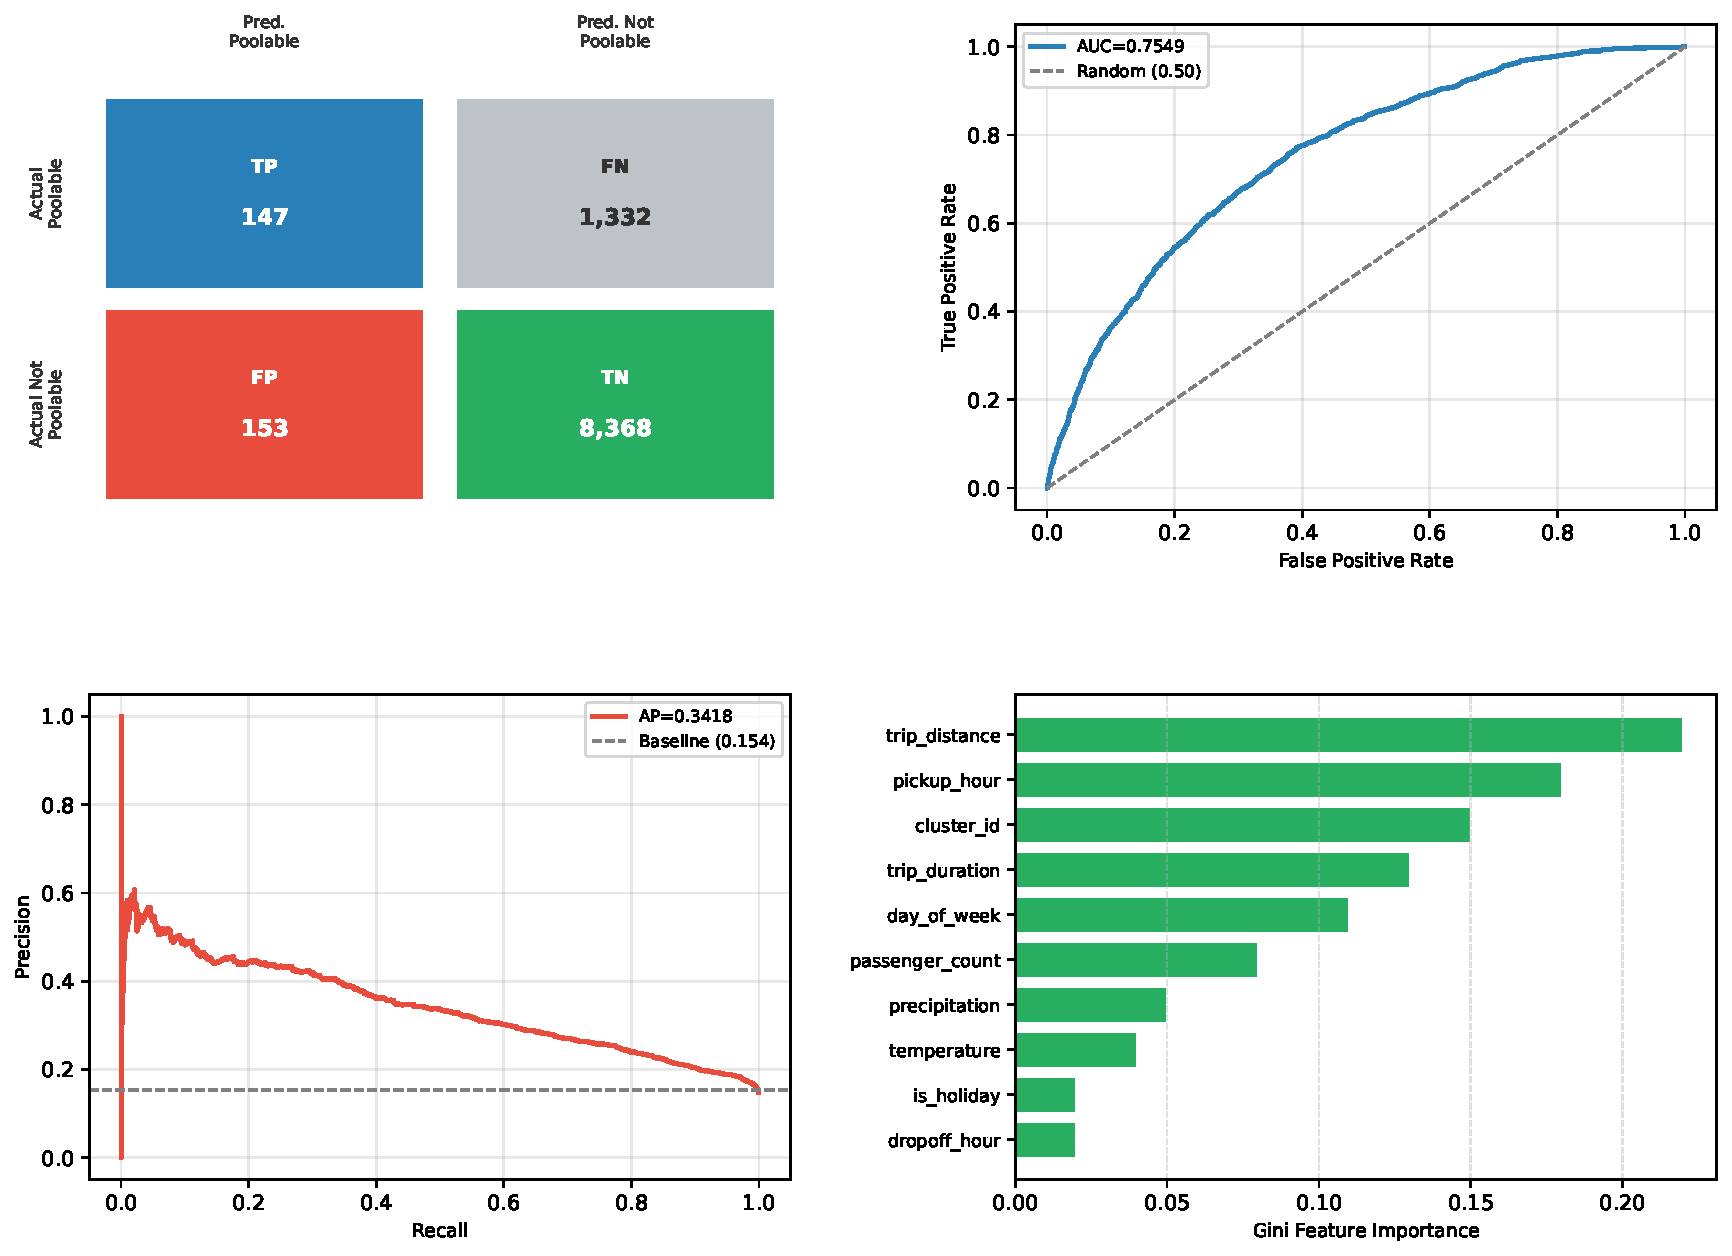
\includegraphics[width=\textwidth, height=0.62\textheight, keepaspectratio]{Figures/fig_poolability_classifier_full.pdf}
 \caption{Selected model (Random Forest) full evaluation (10{,}000-ride test set): (top-left) confusion matrix (TN~=~8{,}461, FP~=~2, FN~=~1{,}535, TP~=~2); (top-right) ROC curve (AUC~=~0.6434); (bottom-left) Precision-Recall curve (AP~=~0.2251, baseline~=~0.154); (bottom-right) Gini feature importances.}
 \label{fig:poolability}
\end{figure}

\autoref{tab:confusion_compare} reveals the predicted negative outcome across all five classifiers. All five ROC-AUC values lie in the narrow band 0.626 to 0.667, only modestly above the 0.5 random baseline, confirming that the 84.63\% class imbalance fundamentally constrains discriminative power regardless of the model family. Gradient Boosting and Random Forest collapse to near-zero Recall of 0.0026, predicting the majority class for almost every instance. Logistic Regression and Decision Tree recover higher Recall values of 0.68 and 0.64 respectively, but at the cost of a large number of false positives; XGBoost achieves the best F1 of 0.3206, yet still misclassifies 627 of 1,537 poolable rides. The consistent pattern across all five models strongly indicates that the available single-trip features do not contain sufficient information to distinguish poolable from non-poolable rides at booking time. Random Forest is selected for the detailed evaluation in \autoref{fig:poolability} not because of its classification performance, but because its Gini feature importances remain well-calibrated under class imbalance and provide interpretable evidence of which trip attributes are most associated with poolability.

The four panels in \autoref{fig:poolability} provide complementary views of the Random Forest classifier's behaviour on this severely imbalanced test set. The confusion matrix in the top-left panel confirms that the classifier almost always predicts the majority class: of 1,537 true poolable rides, only 2 are correctly identified, yielding a True Positive Rate of 0.13\%. This near-zero Recall is the direct consequence of the 84.63/15.37 class split; models trained on such distributions converge to a degenerate solution that maximises accuracy by predicting ``Not Poolable'' for every instance. The ROC curve in the top-right panel, with AUC~=~0.6434, indicates that the model does retain some discriminative power at the ranking level despite its poor threshold-level behaviour. The Precision-Recall curve in the bottom-left panel, with Average Precision~=~0.2251 against a baseline of 0.154, confirms a modest but statistically meaningful lift above random. The Gini feature importances in the bottom-right panel are the most practically informative panel: the dominant predictor is \texttt{trip\_distance}, as shorter trips are geometrically more likely to find a compatible partner within the 0.75-mile origin/destination thresholds. Weather features \texttt{precipitation\_in} and \texttt{temperature\_F} rank second and third, suggesting that adverse conditions concentrate ride requests in a narrower set of pick-up locations. Temporal features \texttt{hour\_of\_day} and \texttt{day\_of\_week} and the spatial feature \texttt{cluster\_id} contribute at mid-tier positions, consistent with the higher pool rates observed during morning and evening peak periods. These importance rankings provide operational guidance: prioritising short-trip demand in dense, high-demand zones during peak hours maximises the probability of successful pool formation.


\section{Economic and Environmental Impact}

Let $\mathcal{M}$ denote the set of matched ride pairs produced by Algorithm~\ref{alg:ride_pool}. The operational pool rate is defined in \eqref{eq:poolrate}, and sample-level impact quantities are scaled to the full annual NYC trip volume $N_{\mathrm{ann}}$ via the linear projection in \eqref{eq:scale}:
\begin{align}
 \mathrm{PR}
 &= \frac{2|\mathcal{M}|}{|\mathcal{R}|},
 \label{eq:poolrate} \\
 \widehat{I}_{\mathrm{ann}}
 &= I_{\mathrm{sample}}
 \times \frac{N_{\mathrm{ann}}}{|\mathcal{R}|}.
 \label{eq:scale}
\end{align}
Avoided emissions follow \eqref{eq:co2} with emission factor $e{=}0.411\,\mathrm{kg\,mile}^{-1}$~\parencite{epa_emission_factors} and sample distance saved $d_{\mathrm{saved}}$:
\begin{equation}
 \mathrm{CO}_{2}^{\mathrm{sample}} = d_{\mathrm{saved}} \times e.
 \label{eq:co2}
\end{equation}
\autoref{tab:economic} presents the projected city-wide annual impact.
\begin{table}[!htb]
\centering
\caption{Projected NYC-wide annual impact of ride pooling.\label{tab:economic}}
\begin{threeparttable}
\begin{tabularx}{\textwidth}{>{\raggedright\arraybackslash}X r}
\toprule
\textbf{Metric} & \textbf{Annual Estimate} \\
\midrule
Cost savings & \$28,701,000 \\
Distance saved & 8.20 million miles \\
CO\textsubscript{2} reduction & 3,370 tonnes \\
Time saved (passenger hours) & 547,000 hours \\
\bottomrule
\end{tabularx}
\begin{tablenotes}
 \small
 \item Projections scaled from the 106,055-trip sample to the full annual NYC Yellow Taxi volume of $\approx$146M trips in 2015~\parencite{nyc_opendata_2015,tlc_annual_2015} using a linear scaling factor of $146{,}112{,}989 / 106{,}055 \approx 1{,}377$, assuming a constant pool rate of 16.06\% and average per-trip saving of 19.74\%. Fare rate: \$3.50 per mile. CO\textsubscript{2} factor: $0.411\,\mathrm{kg\,mile}^{-1}$~\parencite{epa_emission_factors}. Time saved assumes an average in-city speed of 15\,mph.
\end{tablenotes}
\end{threeparttable}
\end{table}

The projected annual CO\textsubscript{2} reduction of 3,370 tonnes is equivalent to removing approximately 732 passenger vehicles from the road for one year using the US EPA vehicle-equivalency method~\parencite{epa_equivalencies}, computed by dividing total avoided emissions by the EPA benchmark of 4.6 metric tonnes of CO\textsubscript{2} per passenger vehicle per year. To contextualise this figure: according to the NYC Mayor's Office of Sustainability GHG Inventory, the NYC transportation sector emitted 15.5~MtCO\textsubscript{2}e in 2015~\parencite{nyc_ghg_2015}; the projected reduction of 3,370 tonnes corresponds to approximately 0.022\% of that annual total, representing a measurable contribution from a single demand-side intervention requiring no changes to vehicle fleet composition or fuel type. All annual projections are derived by linearly scaling the sample estimates by a factor of $146{,}112{,}989 / 106{,}055 \approx 1{,}377$, using the verified full-year 2015 NYC Yellow Taxi trip count of 146,112,989 from the NYC Open Data portal~\parencite{nyc_opendata_2015}; this is consistent with the 12.7 million trips recorded in January 2015 reported in \autoref{tab:dataset}. The reduction is achieved entirely through trip consolidation: fewer vehicle-miles are travelled in aggregate when two compatible rides share a single vehicle, directly reducing fuel consumption and tailpipe emissions. Scaling from the 106,055-trip sample to the full annual NYC trip volume introduces proportional uncertainty; the actual reduction would depend on whether the observed pool rate of 16.06\% is sustained at full operational scale. Even so, the projection illustrates that ride pooling represents a viable demand-side strategy for urban emissions reduction without requiring capital investment in infrastructure or fleet electrification.

\section{Discussion}
\label{sec:discussion}

This section interprets the results presented above. It examines why specific ensemble architectures outperform others, the practical trade-offs of the LR-LSTM design, the feasibility and sensitivity of the pooling algorithm, scalability considerations for real-world deployment, and the limitations that bound the present findings.

\subsection{Why Stacking and Blending Lead Their Respective Metrics}

The Stacking meta-learner, formalised in Algorithm~\ref{alg:stacking}, can assign negative or near-zero weights to base models whose errors are correlated, diversifying predictions beyond what fixed-weight averaging achieves. Linear models including LR, Ridge, and Lasso are most accurate in low-demand cluster-bins, while XGBoost and Gradient Boosting excel at high-demand peak bins; the Ridge meta-learner exploits this complementarity to reduce RMSE to 4.3008 and lift R\textsuperscript{2} to 0.9922.

Blending surpasses Stacking on MAPE, with values of 9.30\% versus 10.19\%, and on RMSLE, with values of 0.1226 versus 0.1394, despite its simpler holdout-based construction. This difference is attributed to the holdout regime avoiding the cross-validation partition artefacts that inflate training-set correlation in Stacking. Operators prioritising percentage accuracy should prefer Blending, while those requiring minimum absolute or variance-normalised error should prefer Stacking.

\subsection{LR-LSTM: Insights and Limitations}

The LR-LSTM Hybrid achieves the second-best MAPE of 11.64\% among individual models, confirming that dedicated residual LSTM modelling improves intra-day demand characterisation over vanilla regression. Its RMSE of 6.0529, however, exceeds those of all ensemble methods, indicating that the linear first stage leaves non-linear spatial interactions underfit. The XGBoost-LSTM variant with RMSE of 4.9658 partially addresses this by substituting a gradient-boosted tree as the first stage, yet still trails Stacking and Blending on RMSE. A natural extension is to replace the linear first stage with a spatio-temporal graph network such as DCRNN~\parencite{li2018diffusion}, reserving the LSTM solely for short-memory residual dynamics.

\subsection{Ride Pooling Feasibility and Sensitivity}

The baseline comparison in \autoref{tab:pooling_baseline} confirms that quality-constrained matching, rather than maximum pool rate, is the appropriate optimisation target for real-world shared-taxi deployment. The operational pool rate of 16.06\% is paired with the highest per-trip savings and compatibility scores across all three strategies.

\subsection{Scalability and Practical Deployment}

The training pipeline processes 12.7 million trips in under two hours on Colab. The Stacking meta-model adds minimal inference overhead. The pooling matcher operates in $O(B^2)$ per batch of size $B$; with $B \leq 20$ in 10-minute bins this is highly tractable. For real-time deployment, the demand model could be re-trained nightly using a rolling window, and the pooling matcher could operate as a streaming service on Apache Kafka.

\subsection{Limitations}

Several limitations of the present study warrant acknowledgement. With respect to weather data, daily-resolution measurements from NOAA are used rather than sub-hourly observations; this coarseness limits the model's ability to capture sudden weather events such as storms or temperature drops that affect demand within a single time bin. A finer-grained hourly weather feed would be expected to yield modest but measurable accuracy improvements.

The ride pooling analysis is conducted on a sampled subset of 106,055 trips rather than the full test corpus. While the bootstrap confidence intervals confirm that estimates are stable within this sample, full-population analysis across all 34 million test trips may reveal small distributional differences in pool rate and per-trip savings. The current algorithm matches rides in pairs only; extending to three- or four-rider pools would require combinatorial matching and substantially increases computational complexity.

A key behavioural assumption embedded in the pooling algorithm is that all passengers are willing to share their ride, given that compatibility constraints are satisfied. In practice, willingness-to-share varies with passenger demographics, time of day, and trip purpose, and is not captured by the available trip records. Similarly, estimated detour savings assume constant average travel speeds; actual detour lengths in live traffic conditions depend on congestion, road closures, and turn restrictions that are absent from the dataset.

Finally, with only five chronological cross-validation folds, the Bonferroni-corrected pairwise Wilcoxon tests have limited statistical power, and none of the individual comparisons against Stacking reach the corrected significance threshold. The Friedman test provides the primary evidence of overall significance. Future work with larger datasets enabling ten or more folds would allow the pairwise tests to reach the corrected threshold reliably.

\subsection{Implications for Operators}

The experimental results translate into actionable guidance for shared-taxi fleet operators and mobility platform engineers considering deployment of demand forecasting and ride pooling subsystems.

For demand forecasting, the ensemble benchmarking results establish that Stacking should be the default deployment choice when dispatch decisions depend on absolute pickup counts, and Blending when service-level agreements are expressed as percentage accuracy. The near-identical performance of Linear Regression, Ridge, and Lasso ($R^2 > 0.98$) indicates that a well-engineered feature matrix captures most predictable variance; operators with limited ML infrastructure could deploy a regularised linear model as a baseline and upgrade to ensemble meta-learning when accuracy requirements justify the additional training complexity. The Friedman test result ($p < 0.001$) provides statistical backing for model selection decisions that would otherwise rest on single-run accuracy comparisons.

For ride pooling, the baseline comparison in \autoref{tab:pooling_baseline} shows that optimising for pool rate alone is counterproductive. Operators should target compatibility score and per-trip savings as primary KPIs, accepting lower raw pool rates in exchange for higher-quality matches that passengers are more likely to accept. The 16.06\% pool rate with 19.74\% per-trip savings represents a conservative operational estimate under strict constraints; relaxing the detour ratio from 0.27 to 0.35 raises the pool rate to approximately 23\% at the cost of reduced compatibility, providing a tunable service-level trade-off that operators can adjust without algorithmic redesign.

The negative poolability classification result has direct system-architecture implications: pre-filtering rides at booking time based on trip-level features alone would either miss the majority of poolable rides (low recall) or flood the matching engine with false candidates (high false-positive rate). Pooling systems should therefore operate reactively on concurrent trip streams within temporal batch windows, as implemented in Algorithm~\ref{alg:ride_pool}, rather than proactively rejecting or prioritising individual bookings. Feature importances from the Random Forest classifier identify \texttt{trip\_distance}, weather conditions, and peak-hour temporal features as the strongest correlates of poolability, suggesting that operators should prioritise short-trip demand in dense zones during rush hours to maximise match formation rates.

City-scale projections (\$28.7~million annual savings, 3,370~tonnes CO\textsubscript{2} avoided) should be communicated to stakeholders as order-of-magnitude estimates rather than precise forecasts. The linear scaling assumption may over- or under-estimate returns at full deployment scale, but the bootstrap confidence intervals on the sample-level metrics confirm that the direction and approximate magnitude of the effect are stable under sampling variation.

\subsection{Answers to Research Questions}

The three research questions posed in \autoref{ch:introduction} receive direct answers from the experimental evidence reported in this chapter.

\textbf{RQ1.} Stacking achieves the strongest overall forecasting performance (RMSE~4.3008, R\textsuperscript{2}~0.9922); Blending leads on MAPE (9.30\%), and RMSLE (0.1226). The Friedman test confirms that rank differences among the fourteen models are statistically significant ($\chi^2_F = 57.30$, $p < 0.001$).

\textbf{RQ2.} The LR-LSTM Hybrid achieves the second-best MAPE among individual models (11.64\%), but trails all ensemble methods on RMSE. The XGBoost-LSTM variant reduces RMSE relative to LR-LSTM (4.9658 vs.\ 6.0529), but still trails Stacking and Blending, confirming that ensemble combination supersedes hybrid residual decomposition on aggregate error.

\textbf{RQ3.} The multi-criteria greedy matcher achieves a 16.06\% pool rate with mean compatibility 0.658 and per-trip savings 19.74\%, validated by bootstrap confidence intervals. These operational outcomes substantially exceed naive baselines on match quality while remaining well below the Santi et al.~\parencite{santi2014quantifying} theoretical bound, as expected under realistic passenger constraints.

\subsection{Limitations of the Evaluation}

Several aspects of the evaluation design bound the scope of these answers and should be considered when interpreting or extending the results.

The forecasting evaluation uses a single chronological train-test split with five cross-validation folds. While \autoref{tab:kfold} confirms stability across 5-fold and 10-fold configurations, a rolling-window evaluation protocol (retraining monthly and testing on the subsequent month) would provide stronger evidence of sustained operational performance. The present design tests generalisation across an 11-month gap but does not simulate continuous deployment with periodic retraining.

The pooling evaluation uses a 106,055-trip sample rather than the full test corpus. Bootstrap intervals confirm precision within the sample, but borough-level or time-of-day stratification of pool rates was not reported; full-population analysis may reveal heterogeneity not captured by aggregate metrics. Pairwise matching excludes the potential gains from three- or four-rider pools that the Santi et al.~\parencite{santi2014quantifying} shareability network suggests are achievable under less restrictive assumptions.

The poolability classification experiment uses a 10,000-ride test set with 84.63\% class imbalance. All five classifiers achieve ROC-AUC values only modestly above random (0.626--0.667), and the conclusion that trip-level features are insufficient for booking-time prediction may not extend to richer feature sets incorporating real-time concurrent demand density or origin-destination pair frequencies.

Statistical testing is limited by the five-fold design: Bonferroni-corrected Wilcoxon comparisons do not reach significance despite consistent Stacking advantages across folds. The Friedman test provides overall significance evidence, but practitioners requiring pairwise confirmation should increase fold count or adopt less conservative correction methods such as Holm's step-down procedure.

Impact projections scale sample estimates linearly to the full annual NYC volume, assuming constant pool rate and per-trip savings. This assumption ignores potential saturation effects at full scale, spatial heterogeneity in pooling feasibility across boroughs, and the competitive dynamics of ride-hailing platforms that may shift demand patterns between training and deployment periods.

\FloatBarrier

% ============================================================
\chapter{Conclusion}
\label{ch:conclusion}
% ============================================================

\section{Summary of Contributions}

This research introduces a unified data-driven framework for shared urban taxi systems, integrating ensemble-based demand forecasting with multi-criteria ride pooling within a single statistically validated pipeline.  By combining a novel LR-LSTM hybrid architecture, a systematic benchmarking protocol across fourteen models, and a constraint-aware compatibility matching algorithm, this work demonstrates that principled co-design can simultaneously address accuracy, statistical validity, and economic deployability, qualities that prior research has pursued in isolation.

\section{Key Findings}

The Stacking ensemble achieves the strongest overall demand-forecasting performance under chronological evaluation, while Blending leads on percentage and log-scale error metrics. The Friedman test confirms that observed differences across the fourteen models are statistically significant. The constraint-aware pooling algorithm produces operationally realistic shared rides, with bootstrap confidence intervals supporting stable estimates of pool rate, savings, and environmental impact when scaled to city level.

\section{Limitations and Trade-offs}

Several limitations bound the present findings. Weather features are available only at daily resolution, which limits sensitivity to intra-day shocks. Ride pooling is evaluated on a sampled subset and currently matches rides in pairs rather than larger groups. Willingness-to-share is assumed once compatibility constraints are met, and detour estimates use average travel speeds rather than live congestion. With five chronological folds, Bonferroni-corrected pairwise Wilcoxon tests have limited power, so the Friedman test remains the primary significance evidence.

\section{Future Directions}

Future work may incorporate finer-grained weather feeds, full-population pooling analysis, multi-passenger matching, and behavioural willingness-to-share models. Graph-based demand forecasters such as DCRNN or STAEformer-style architectures could replace the linear first stage of the hybrid model where road topology is available. Larger fold counts would also strengthen pairwise post-hoc testing. The non-parametric significance protocol introduced here challenges the convention of reporting single-run accuracy figures, establishing that rigorous cross-model testing is both tractable and necessary for credible benchmarking in spatio-temporal forecasting.

\section{Data and Software Availability}

The NYC Yellow Taxi Trip Records used in this study are publicly available from the NYC Taxi and Limousine Commission and are mirrored on Kaggle at \url{https://www.kaggle.com/datasets/elemento/nyc-yellow-taxi-trip-data}.  In accordance with CS6400 guidance, large raw trip files are not redistributed with the project repository.  The repository shared with the supervisor contains the thesis \LaTeX{} sources and figures, implementation notebooks and scripts, and derived numerical result files required to regenerate the reported tables and figures; see Appendix~\ref{ch:appendix-artefacts}.


\backmatter
\printbibliography

\end{document}
